\begin{refsection} 
 
\chapter{Li-ion Batteries}~\label{chapter:batteries} 
 
\setlength{\epigraphwidth}{3in} 
\epigraph{\textit{``Solar and battery go together like peanut butter and 
jelly.” }}{Elon Musk} 
\vspace{3em} 
 
Since their commercialization in 1991 by Sony, Lithium-ion batteries have 
become one of the most popular type of rechargeable batteries used in portable 
electronics and electric vehicles. Despite their success, Li-ion batteries 
still can benefit significantly from improvements in order to expand their use in 
automotive and grid storage applications. One of the main elements of the 
Li-ion battery with room for improvement is the cathode, where research is primarily 
focused on layered transition metal (TM) oxides and polyanionic materials.  
 
In this chapter I present an overview of my work on Li-ion batteries, which 
has largely focused on a class of materials called Li-rich battery cathodes. 
The chapter starts with a brief introduction on the topic of Li-ion 
batteries in Section~\ref{batteries:sec-intro}. Next, 
Section~\ref{batteries:sec-lirich} introduces \ce{Li}-rich materials and 
presents an analysis of the structure and \ce{Li}-configuration 
(Sec.~\ref{batteries:sec-structure}), the redox processes 
(Sec.~\ref{batteries:sec-oxidation}) and dimer formation 
(Sec.~\ref{batteries:sec-dimer}). Section~\ref{batteries:sec-substitutions} concerns the solubility of \ce{Sn} 
in \ce{Li2MnO3} (Sec.~\ref{batteries:sec-Sn_stability}) as well as the 
influence of a local substitution of \ce{Sn}, \ce{V} and \ce{Mo} on the 
stability of the oxygen framework 
(Sec.~\ref{batteries:sec-dimer_substitution}). Finally, 
Section~\ref{batteries:sec-solid_electrolyte} briefly introduces solid 
electrolytes, as well as a promising class of materials called 
polyborane salts (Sec.~\ref{batteries:sec-polyborane_salts}) and the 
calculation of their local cation energy landscape 
(Sec.~\ref{batteries:sec-landscape}).
 
\clearpage 
 
\section{Introduction} \label{batteries:sec-intro} 
 
Energy storage is one of the most important topics of our contemporary 
society. From portable electronics to the transportation sector, the storage 
of electrical energy plays a vital role in many aspects of our daily lives. 
Moreover, it is an essential component of the transition to renewable energy, 
as many renewable sources of energy are intermittent, requiring the storage of 
excess energy to stabilize the grid. Ranging from something as simple as 
pumping water to a higher elevation\footnote{Although simple, this is arguably 
still one of the best ways to store energy for grid applications. A good 
example is our very own hydrostorage facility at Coo, which professes to have 
an energy conversion efficiency of 75\%~\cite{Engie-Electrabel2015}.} to 
storing superconducting magnetic energy storage, there are many methods for 
storing energy. Which storage solution is optimal depends largely on the 
application. In portable electronics and the electrical vehicle (EV) market, 
Li-ion batteries have been used extensively as the energy storage medium of 
choice. 
 
Li-ion batteries consist of two electrodes with different chemical potentials 
for \ce{Li^+}, separated by an electrolyte (Fig.~\ref{batteries:fig-li_ion}). 
When the battery is charged or discharged, \ce{Li^+} ions move between the two 
electrodes through the electrolyte, while electrons flow in the same direction 
via an external circuit in order to maintain charge balance. Although which 
electrode functions as a cathode or anode depends on whether the battery is 
being charged or discharged, it is the convention to stick to the standard 
terminology used during the charging process. That is, the cathode delivers 
electrons to the external circuit as the battery is charged. At the same time, 
\ce{Li^+} ions move to the anode, which means that for a fully charged 
\ce{Li}-ion battery, as much \ce{Li} as possible should be stored in the 
anode. Using this convention, the chemical potential for \ce{Li^+} should be 
higher for the anode than the cathode to ensure that \ce{Li^+} ions and 
electrons spontaneously move to the cathode when the battery is discharged. 
 
\begin{figure}[ht] 
\centering 
\captionsetup{width=0.8\linewidth}
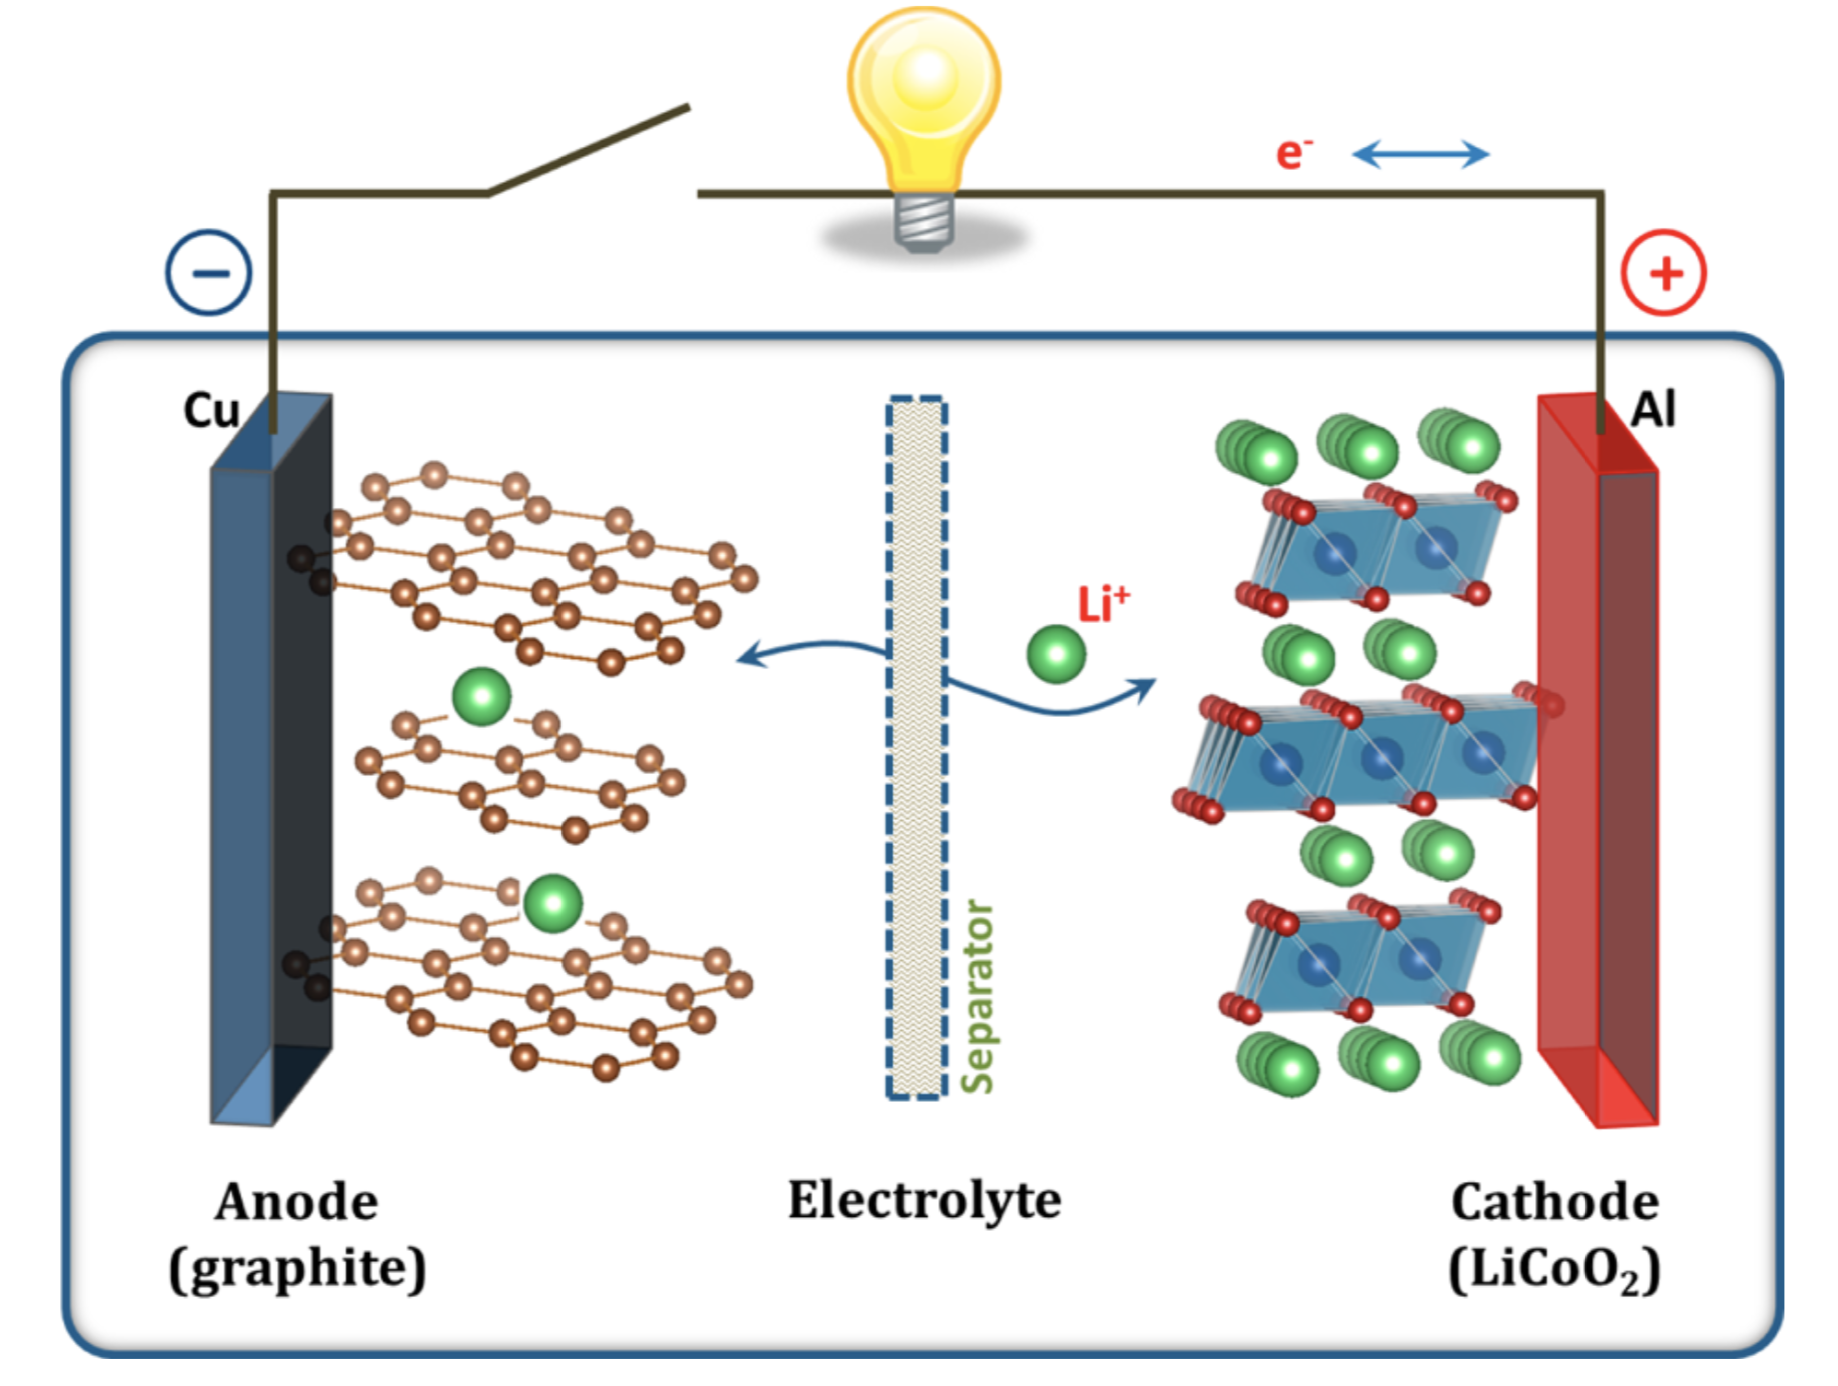
\includegraphics[width=0.7\textwidth]{./figures/batteries/li-ion_battery.png} 
\caption{Basic composition of a Li-ion battery~\cite{Goodenough2013}.} 
\label{batteries:fig-li_ion} 
\end{figure}
 
% When choosing materials for batteries, there are several important properties 
% to consider. First is the ability of the material for storing Li-ions which is 
% best expressed as the specific capacity. # TODO?
 
For the anode, most commercially available \ce{Li}-ion batteries use graphite 
due to its low price, weight and relatively large specific capacity of 
372~\si{\milli\ampere\hour/\gram}~\cite{Mao2018}. Moreover, its layered 
structure is remarkably stable, leading to  a high reversibility and 
cyclability. For the cathode, a more diverse set of materials is being 
considered. The conventional layered oxides \ce{LiMO2}, where \ce{M} is a 
(combination of) transition metals, is still one of the most popular 
chemistries due to their high energy density and rate capacity~\cite{Bresser2015}. Spinel-type 
oxygen-based cathodes~\cite{Thackeray2004} (e.g. \ce{LiMn2O4}) have a lower capacity compared to 
the layered oxides, but are also receiving a fair bit of attention because of 
their excellent safety. Similarly, ordered olivine compounds~\cite{Padhi1997} (e.g. \ce{LiFePO4}) are lauded for their 
high safety and structural stability, but suffer from a reduced specific 
capacity due to their high weight. The electrolyte separating the electrodes 
can be either a liquid or a solid, 
with the liquid being the conventional choice owing to its high ionic 
conductivity. However, there are certain safety hazards associated with the 
use of liquid electrolytes. 

\section{Li-Rich Battery Cathodes} \label{batteries:sec-lirich} 
 
Li-ion batteries are currently the primary method of energy storage for many 
important applications, however many potential gains in energy density can 
still be made by improving the cathode capacity. Layered \ce{LiMO2} compounds, 
where \ce{M} is a transition metal, allow for fast two dimensional lithium 
diffusion through a divacancy mechanism~\cite{VanderVen2001}, and high 
voltages versus the battery anode. Among this group, \ce{LiCoO2} has long been 
the favoured cathode in commercial applications. Cobalt is expensive and 
toxic, however, and suffers from safety problems due to its low thermal 
stability~\cite{Larcher2015}. Moreover, the capacity of \ce{LiCoO2} is limited 
to 130~\si{\milli\ampere\hour/\gram}, because only about half of the lithium 
can be extracted without causing severe electrode 
degradation~\cite{Rozier2015}. 
 
\begin{figure}[ht] 
\centering 
\captionsetup{width=0.9\linewidth}
\includegraphics[width=\textwidth]{figures/batteries/to_li_rich.png} 
\caption{Transition from \ce{LiCoO2} to NMC to Li-rich layered oxides for 
battery cathodes. Adapted from~\cite{Rozier2015}.} 
\label{batteries:fig-Lirich_transition} 
\end{figure} 
 
In order to improve upon these deficiencies, material scientists have 
attempted chemical substitution of Co by other transition metals such as 
\ce{Mn} and \ce{Ni} (Fig.~\ref{batteries:fig-Lirich_transition}). Since 
\ce{LiNiO2} is deemed unsafe because of its low thermal 
stability~\cite{Ohzuku1993} and \ce{LiMnO2} suffers from poor electrochemical 
performance~\cite{Vitins1997}, researchers use partial substitution of Mn and 
Ni in \ce{LiCoO2} to fine-tune the qualities of the cathode 
material~\cite{Koyama2003}. The resulting \ce{Li[Ni_{1-x-y}Mn_xCo_y]O2} (NMC) 
compounds show improved capacities (200~\si{\milli\ampere\hour/\gram}) and 
safety characteristics, without significantly changing the operating 
voltage~\cite{Zhou2011}.  
 
More recently, further explorations on layered oxide structures have led to 
Li-rich materials, which have an excess of Li in the material 
composition~\cite{Thackeray2007} (Fig.~\ref{batteries:fig-Lirich_transition}). 
These compounds can attain even higher capacities. The origin of this extra 
capacity is believed to be anionic reversible redox processes (\ce{O^{2-}} → 
\ce{O2^{2-}})~\cite{Sathiya2013}, which changes the fundamental minimum of 
transition metal content that was considered necessary in layered oxides for 
decades, and could lead to the next generation of high energy density Li-ion 
batteries. However, these materials still suffer from structural degradation 
as the battery is cycled, reducing the average voltage and capacity of the 
cell. The voltage fade is believed to be related to the migration of 
transition metals into the lithium layer, linked to the formation of O-O 
dimers with a short bond length, which in turn is driven by the presence of 
oxygen holes due to the participation of oxygen in the redox process. Finally, 
the \ce{Li}-rich cathodes have also demonstrated oxygen evolution from the 
structure as the battery is charged, which is detrimental for the safety of 
battery. 
 
This section presents an investigation into the connection between oxygen 
redox and the stability of the oxygen framework for \ce{Li}-rich materials, 
based on \ce{Li2MnO3} and \ce{Li2IrO3}. These two \ce{Li}-rich cathode 
materials have demonstrated significantly different cycling properties. 
\ce{Li2MnO3}, a well studied \ce{Li}-rich material, suffers from a substantial 
amount of voltage fade as the battery is cycled~\cite{Croy2014}, whereas 
\ce{Li2IrO3} does not~\cite{McCalla2015}. Studying the differences in 
oxidation and structural stability between these two compounds can offer 
insight as to why their cycling properties are so different.  
 
\resultsubsection{Structure and Li configuration \label{batteries:sec-structure}}{https://github.com/mbercx/phd-thesis/tree/master/jupyter/batteries\#structure-and-li-configuration}{structure} 

In order to compare the structural stability of the oxygen framework for the 
\ce{Li2MnO3} and \ce{Li2IrO3} compounds, we have to calculate the chemical 
reaction energy for the formation of O-O dimers for both cathode materials in 
a charged state, i.e. after the removal of a certain fraction of lithium. 
However, the fully charged structure for \ce{Li2MnO3} is found to be highly 
unstable, i.e. lead to the spontaneous formation of several oxygen dimers, 
especially when any local changes to the structure are made. Moreover, the 
cathode is unlikely to ever be fully delithiated in a practical battery, 
rendering an investigation of the fully charged state less relevant. 

\begin{figure}[ht] 
\centering 
\captionsetup{width=0.9\linewidth}
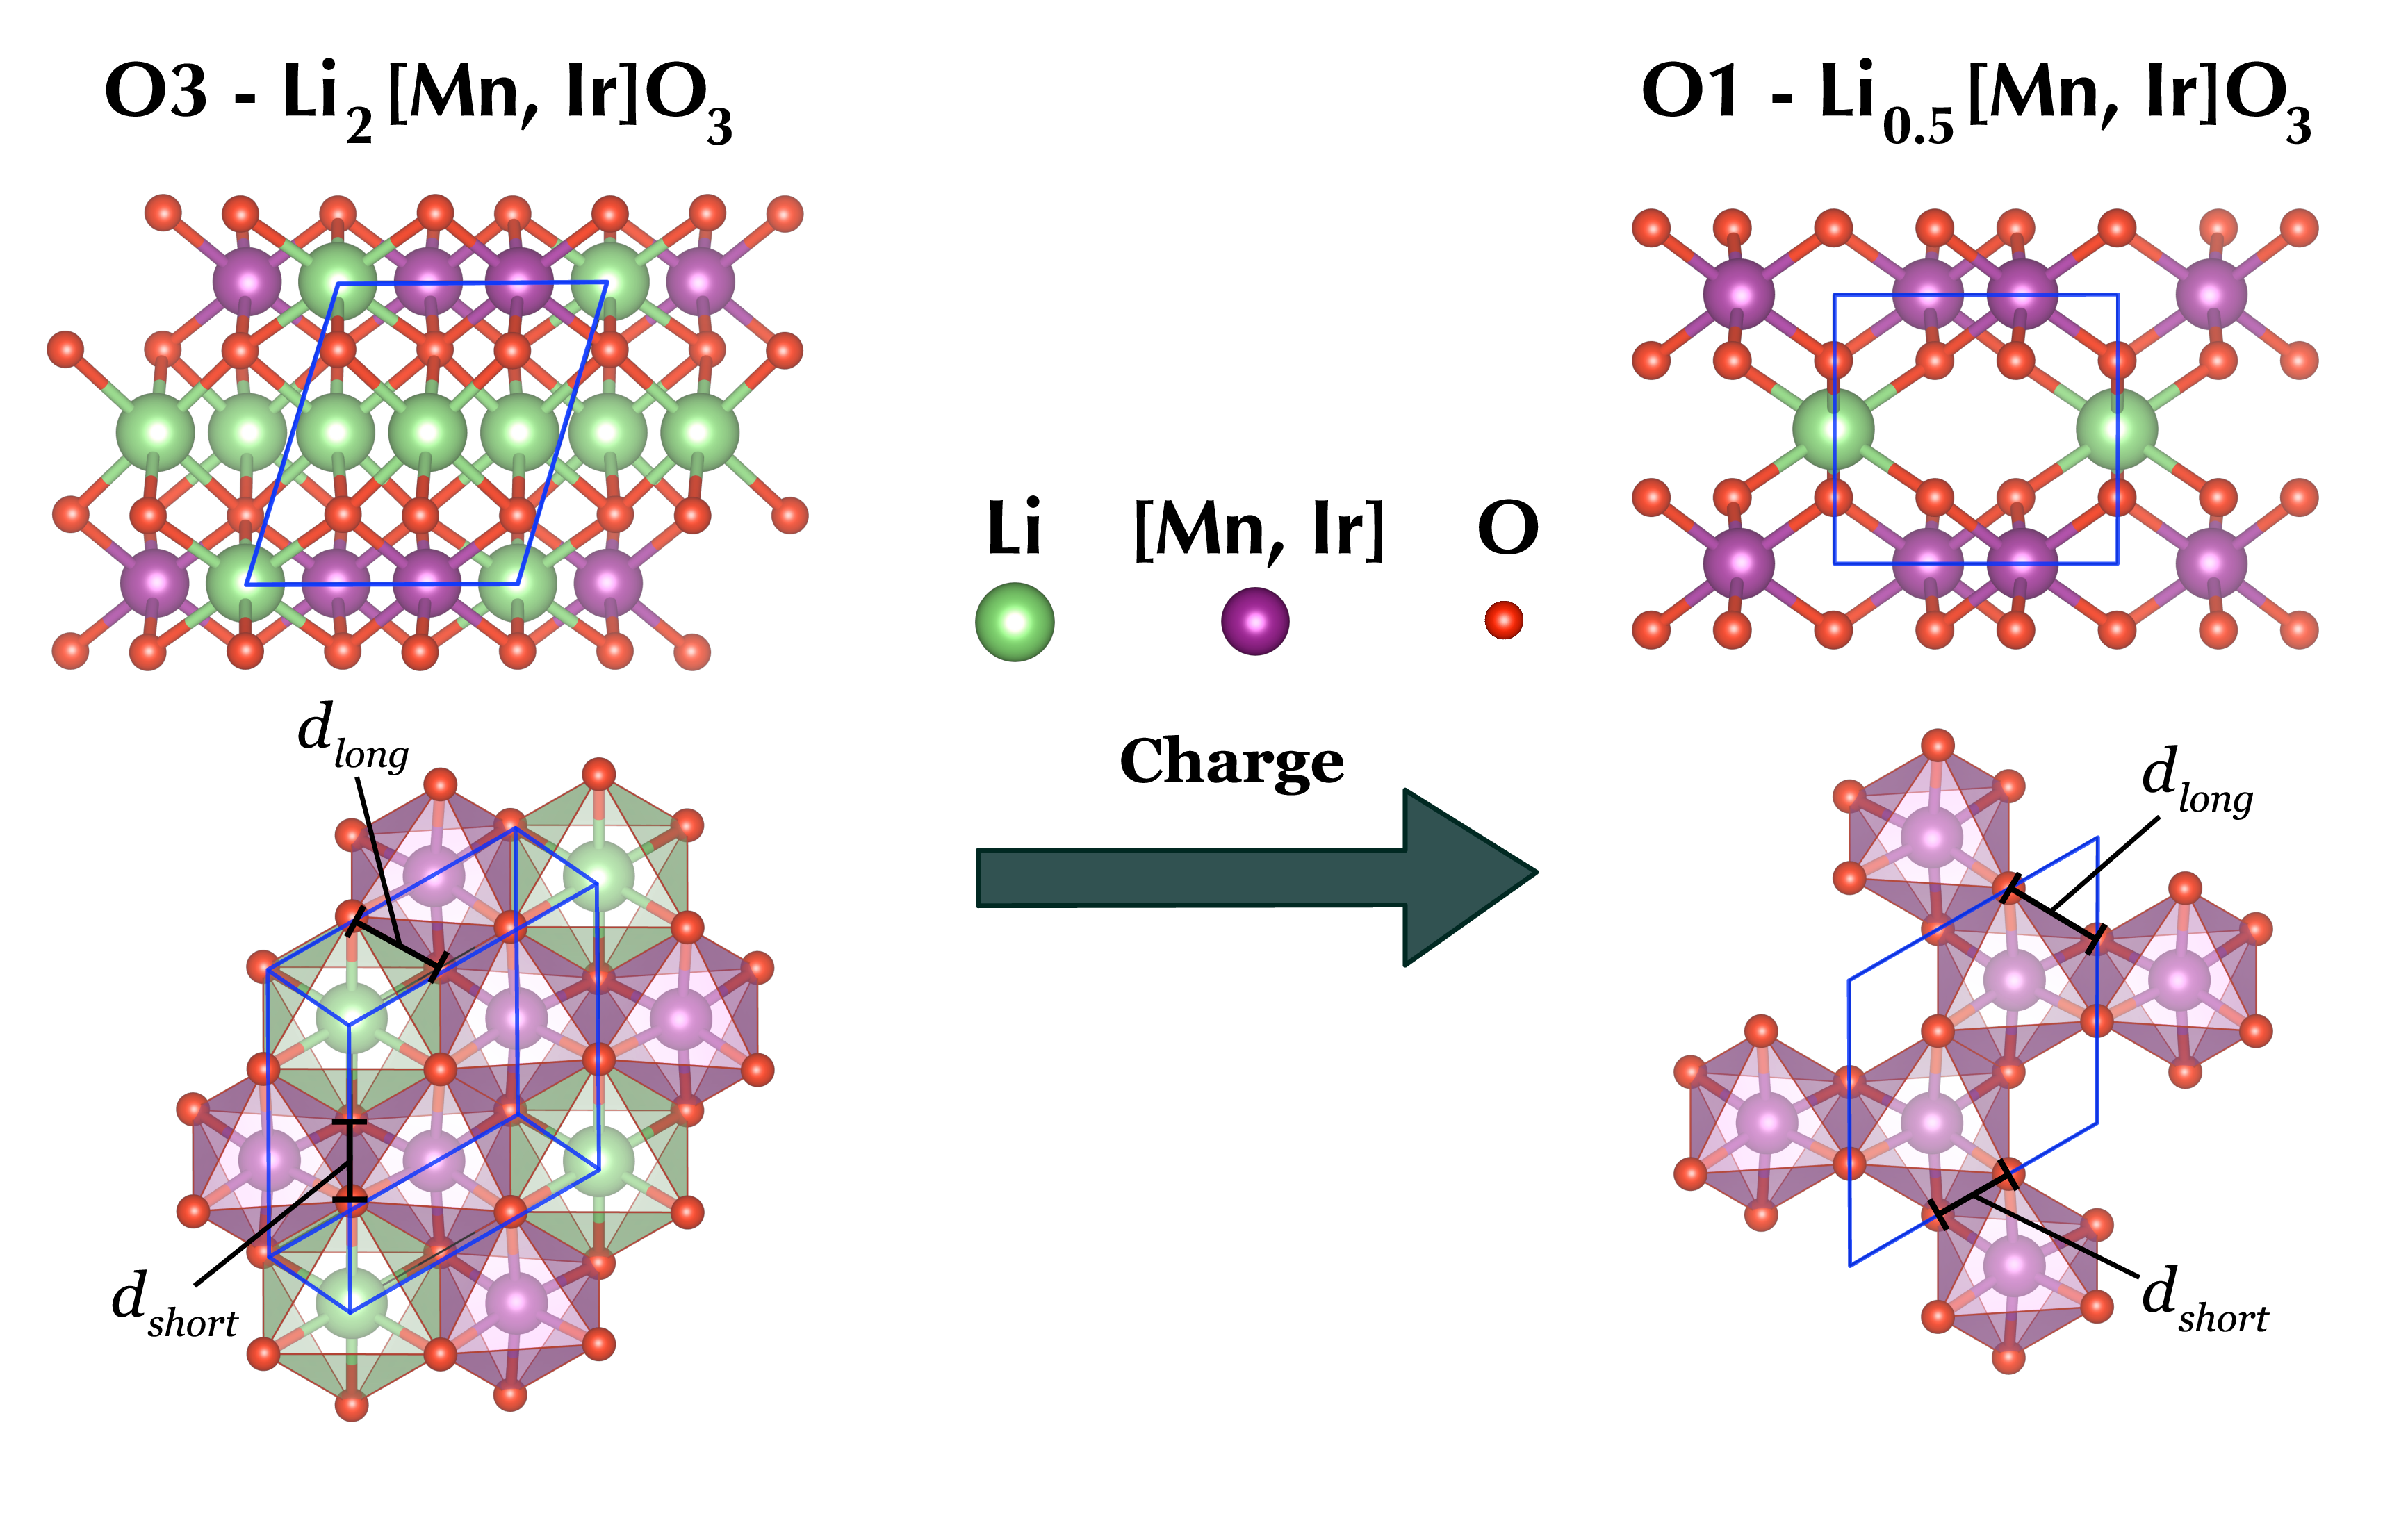
\includegraphics[width=0.9\textwidth]{figures/batteries/structural_change.png} 
\caption{Transformation from the O3 to O1 stacking for both \ce{Li2MnO3} and 
\ce{Li2IrO3} as the cathode is charged. The primitive unit cell 
is drawn in blue. The top figures are the structure shown in the [100] 
projection, whereas the lower figures represent a single octahedral layer of 
the layered structure, viewed top down.  $d_{short}$ and $d_{long}$ both 
represent O-O distances across the \ce{Li}/TM layer, corresponding to an 
octahedral edge bordering two TM's and a TM and \ce{Li}/Vacancy, respectively.} 
\label{batteries:fig-structural_change} 
\end{figure} 

Hence, the structural stability should preferably be studied in a partially 
charged cathode material. This requires knowledge about the location of the 
lithium for each state of charge, as there are many possible \ce{Li}-Vacancy 
configurations to consider. We investigate the lithium configuration for 
\ce{Li2MnO3} by calculating the energy of all symmetrically non-equivalent 
configurations in the conventional unit cell. This is done based on the 
workflow described in Section~\ref{automation:sec-configurations}, resulting 
in 94 non-equivalent configurations. Similar to previous 
work~\cite{Koyama2009}, we find that for the several lithium configurations, 
the \ce{Li2MnO3} structure spontaneously shifts from an O3 stacking to the O1 
stacking\footnote{The various stackings of layered oxides were first classified 
by Delmas et al.~\cite{Delmas1980}. O refers to the octahedral coordination 
of O atoms around the alkali (Li, Na, ...) ions. The number is related to 
the stacking of the O atoms, i.e. for O3 the stacking is AB CA BC, so after 
3 layers of alkali ions, the oxygen environment returns to its original 
stacking. For O1, the stacking is AB AB, so the stacking for each alkali 
layer is the same.} at higher charge state of the battery 
(see Fig.~\ref{batteries:fig-structural_change}). In order to verify this transition from 
the O3 to the O1 stacking, we once again use the configuration workflow to 
calculate the energy of all \ce{Li} configurations in unit cells up to two 
times the size of the conventional unit cell of the O1 stacking, which results 
in 220 non-equivalent configurations. 

For the O1 stacking, we find that 
several configurations at lower states of charge switch to the O3 stacking, 
i.e. the opposite transformation occurs compared to that at higher states of 
charge. To be able to compare the energies of the O1 and O3 stackings fairly, we 
remove the configurations which change stacking. As the stacking 
of the oxygen octahedra is closely connected to the angles between the 
lattice vectors, we remove all configurations for which any lattice angle has 
changed more than 12\si{\degree}. This leaves 84 and 181 configurations for 
the O3 and O1 stacking, respectively. Finally, we calculate the formation 
energy for all configurations versus the fully charged and discharged state of 
the O3 stacking: 
\begin{equation} 
E_f (x) = E(\ce{Li_xMnO3}) - (1 - \frac{x}{2}) E(\text{O3-}\ce{MnO3}) - 
\frac{x}{2} E(\text{O3-}\ce{Li2MnO3}) 
\end{equation} 
The corresponding formation energies are plotted for both stackings in 
Fig.~\ref{batteries:fig-li_configuration}. It is clear that as \ce{Li} is 
removed from \ce{Li2MnO3}, the O1 stacking becomes thermodynamically 
favorable. 
 
\begin{figure}[ht] 
\centering
\captionsetup{width=0.9\linewidth}
\includegraphics[width=0.7\textwidth]{figures/batteries/o1_vs_o3.png} 
\caption{Formation energies of all configurations in both the O3 and O1 
stacking of \ce{Li_xMnO3}. Each mark represents the formation energy of one non-equivalent Li configuration. The full lines correspond to the convex hull of the 
corresponding stacking.} 
\label{batteries:fig-li_configuration} 
\end{figure} 
 
A similar transformation from the O3 to O1 stacking is found to occur for 
\ce{Li_{0.5}IrO3}, which has been experimentally verified and leveraged in 
order to study the deformation of the oxygen framework by McCalla et 
al.~\cite{McCalla2015}. This means that structures of the discharged and 
charged structures are the same, save for a difference in the lattice 
parameters, which facilitates the comparison of the changes in geometry and 
oxidation state between \ce{Li2MnO3} and \ce{Li2IrO3}. We choose to focus on 
the 75\% charged structures for several reasons. First, the optimal lithium 
configuration for \ce{Li_{0.5}MnO3} is on the convex hull of the O1 stacking, 
indicating that this structure is quite stable and hence easier to work with 
once we start introducing O-O dimers (Sec.~\ref{batteries:sec-dimer}). Second, 
oxygen gas is only released from the \ce{Li2IrO3} cathode once it is charged 
beyond 75\%~\cite{McCalla2015}, whereas \ce{Li2MnO3} has already lost oxygen at this state of 
charge~\cite{Castel2014}. Hence, studying the stability for this lithium content is most 
interesting, as it may show discrepancies between the stability of the oxygen 
frameworks. Finally, the oxygen framework of \ce{Li_{0.5}IrO3} was studied by 
McCalla et al.~\cite{McCalla2015}, which allows for a direct comparison of our 
calculated O-O distances with experiment. 

\begin{table}[ht] 
\centering 
\captionsetup{width=0.9\linewidth}
\renewcommand{\arraystretch}{1.3} 
\caption{O-O distances for the dicharged and charged \ce{Li2[Mn, Ir]O3} 
structures, all expressed in \AA. The distances for \ce{Li2IrO3} are compared 
with the neutron powder diffraction results of McCalla et 
al.\cite{McCalla2015}.} 
\label{batteries:tab-OO_distance} 
\begin{tabular}{c c c c c c c} 
 & & \multicolumn{2}{c}{\ce{Li2[Mn, Ir]O3}} & & 
\multicolumn{2}{c}{\ce{Li_{0.5}[Mn, Ir]O3}}\\\cline{3-4}\cline{6-7} 
 & & DFT & Neutron & & DFT & Neutron \\\hline 
\multirow{2}{*}{Mn} & \multicolumn{1}{|c}{$d_{short}$} & 2.52 & - & & 2.31 & - 
\\ 
 & \multicolumn{1}{|c}{$d_{long}$} & 2.75 & - & & 2.62 & - \\\hline 
\multirow{2}{*}{Ir} & \multicolumn{1}{|c}{$d_{short}$} & 2.75 & 2.77 & & 2.51 
& 2.54 \\ 
 & \multicolumn{1}{|c}{$d_{long}$} & 2.87 & 2.84 & & 2.74 & 2.77 \\\hline 
\end{tabular} 
\end{table} 
 
As was noted previously by McCalla et al.~\cite{McCalla2015}, the oxygen 
framework is distorted as lithium is removed from the structure. In order to 
quantify this, we determine the distances between the various oxygen pairs, 
connected in the tetrahedral environment of \ce{Mn} or \ce{Ir}. The distances 
between oxygen pairs which are part of the same oxygen layer change little. 
However, for the interlayer oxygen pairs, denoted as $d_{short}$ and 
$d_{long}$ in Figure~\ref{batteries:fig-structural_change}, the change in bond 
length is more pronounced (Table~\ref{batteries:tab-OO_distance}). Moreover, 
the shorter bonds for an oxygen pair sharing two [Mn, Ir] neighbors, shrink 
more than the long bonds, which share a transition metal and Li or vacancy. 
This leads to a distortion of the octahedral environment around the transition 
metals, resulting in short O-O bonds which McCalla et al. refer to as dimers. 
In Section~\ref{batteries:sec-dimer}, we will return to this topic, focussing 
our attention on the formation of a peroxo species with a bond length closer 
to that of the oxygen molecule, as this formation has been derived 
theoretically for \ce{Li2MnO3}, and believed to be related to the migration of Mn 
and the resulting voltage fade~\cite{Chen2016}. 
 
% Atomic orbital diagrams are also drawn in order to elucidate the connection 
% between the magnetic moment and the oxidation state for Mn and O.  
 
\resultsubsection{Oxidation \label{batteries:sec-oxidation}}{https://github.com/mbercx/phd-thesis/tree/master/jupyter/batteries\#oxidation}{oxidation} 
 
Sathiya et al.~\cite{Sathiya2013} have discussed that removing lithium from 
\ce{Li}-rich cathodes leads to the formation of holes on the oxygen, i.e. the 
oxidation of oxygen. Seo et al.~\cite{Seo2016} have proposed that the 
formation of localized holes relies on the presence of labile oxygen states, 
which are found for oxygen with \ce{Li} atoms on opposite sites of its 
octahedral environment. Moreover, they explain that because of the honeycomb 
structure of \ce{Li2MnO3}, all oxygen environments have such a 
\ce{Li}-\ce{O}-\ce{Li} configuration, leading to a high participation of 
oxygen in the redox processes. Although \ce{Li2IrO3} has a similar structure, 
Hong et al.~\cite{Hong2019} assert that because \ce{Ir^{4+}} can be more 
easily oxidized, these labile oxygen states are not depleted to the same 
extent, stabilizing the oxygen framework. 
 
\begin{table}[ht] 
\centering
\captionsetup{width=0.9\linewidth}
\renewcommand{\arraystretch}{1.3} 
\caption{Calculated absolute values of the magnetic moments for the discharged 
and charged \ce{Li2[Mn, Ir]O3} structures, all expressed in Bohr magnetons $\mu_B$. Note that 
for the \ce{Ir} structures, non-collinear calculations were performed to include spin-orbit coupling, and the norm of the local magnetization vector was calculated in order to 
express the local magnetic moment as a scalar.} 
\label{batteries:tab-magmoms} 
\begin{tabular}{c c c c} 
 & & \ce{Li2[Mn, Ir]O3} & \ce{Li_{0.5}[Mn, Ir]O3} \\\hline 
\multirow{2}{*}{Mn} & \multicolumn{1}{|c}{$|\mu|$ (\ce{Mn})} & 2.918 & 2.949 
\\ 
 & \multicolumn{1}{|c}{$|\mu|$ (\ce{O})} & 0.001 & 0.445  \\\hline 
\multirow{2}{*}{Ir} & \multicolumn{1}{|c}{$|\boldsymbol{\mu}|$ (\ce{Ir})} & 0.374 & 1.025 
\\ 
 & \multicolumn{1}{|c}{$|\boldsymbol{\mu}|$ (\ce{O})} & 0.025 & 0.314 \\\hline 
\end{tabular} 
\end{table} 
 
To study the change in the oxidation state of the atoms, we compare the 
calculated local magnetic moments of the various elements for both structures 
in the discharged and 75\% charged state in Table~\ref{batteries:tab-magmoms}. 
Note that as \ce{Ir} exhibits strong spin-orbit coupling effects, non-collinear 
calculations were performed for both \ce{Li2IrO3} and \ce{Li_{0.5}IrO3}.
We can see that for \ce{Li2MnO3}, the magnetic moment of Mn remains largely 
the same, whereas the magnetic moment on oxygen increases significantly. For 
oxygen, the increase in magnetic moment corresponds to an oxidation from its 
\ce{O^{2-}} state, as its $p$-orbitals are no longer fully occupied, leading 
to an increased local density of unpaired electrons. The results for \ce{Mn} 
indicate that it does not participate much in the redox processes that occur 
when the battery is charged. Instead, its magnetic moment remains close to 3 
$\mu_B$, which corresponds to the initial oxidation state \ce{Mn^{4+}} in the 
discharged cathode structure. For \ce{Li2IrO3}, removing lithium from the 
discharged structure results in a significant change of the local magnetic 
moment for both Ir and O, implying a more mixed redox process during the 
charging of the cathode. This mixed redox for \ce{Li2IrO3} is in agreement 
with the XPS results of McCalla et al.~\cite{McCalla2015}, where they explain 
that this is in part due to the covalent character of the Ir-O bond. This 
covalency could also explain why oxygen is oxidized less when charging 
\ce{Li2IrO3}, as valence electrons are removed from both Ir and O. 
\ce{Mn^{4+}} could in principle also be oxidized further, but the \ce{Mn^{5+}} 
oxidation state is rare, and generally not octahedrally 
coordinated~\cite{Saint2007}. The fact that the change in magnetic moment on O 
is smaller for \ce{Li2IrO3}, than for \ce{Li2MnO3} indicates that the mixed 
redox process in the charging of \ce{Li2IrO3} results in a lower state of 
oxidation for the oxygen of the structure in the charged state.  
 
\begin{figure}[ht] 
\centering 
\captionsetup{width=0.9\linewidth}
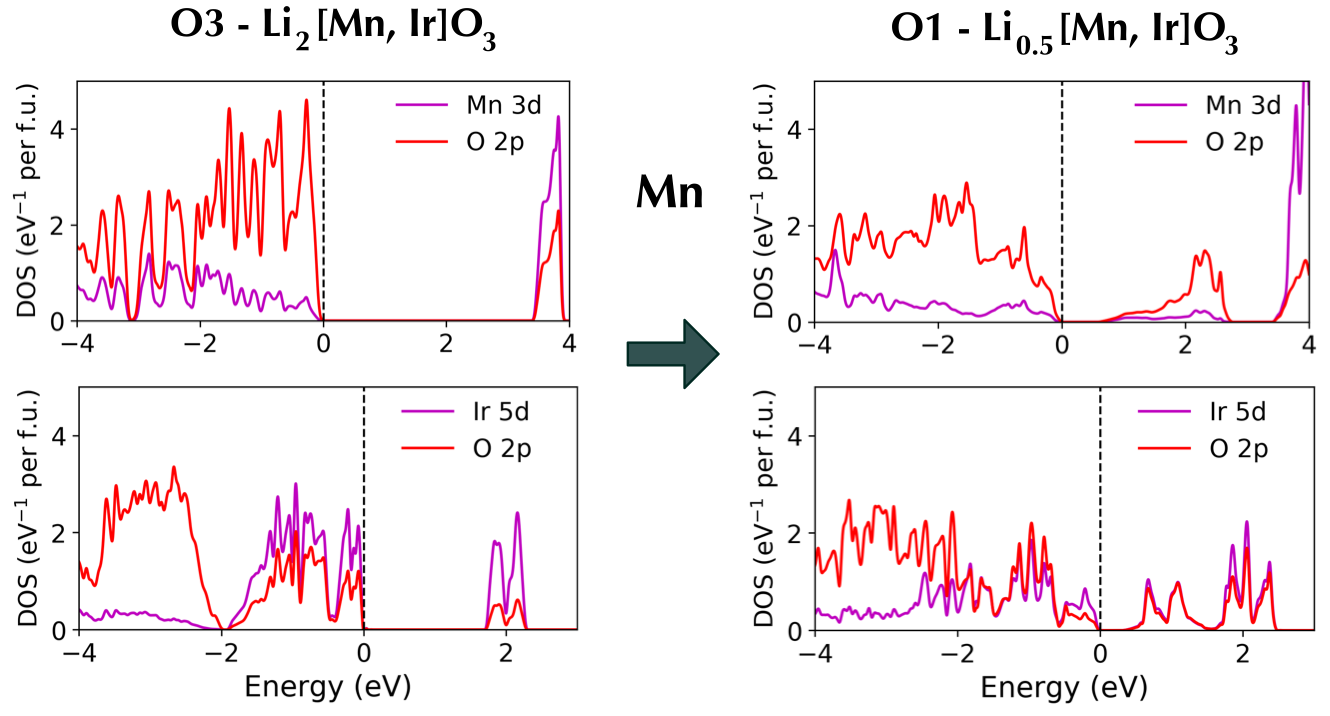
\includegraphics[width=\textwidth]{Figures/batteries/charge_pdos_Mn_Ir.png} 
\caption{The projected density of states of the Mn-3$d$, Ir-5$d$ and O-2$p$ 
orbitals for the discharged (left) and charged (right) structures, where we 
have aligned the Fermi level to zero. In order to allow for a reasonable 
comparison between the pristine and charged state, we have consistently 
plotted the number of states per electronvolt per formula unit.} 
\label{batteries:fig-charge_pdos_Mn_Ir} 
\end{figure} 
 
This conclusion is supported by the projected density of states (PDOS), 
plotted in Figure~\ref{batteries:fig-charge_pdos_Mn_Ir}. For \ce{Li2MnO3}, the 
electronic states close to the Fermi level correspond largely to the O-2$p$ 
states, which indicates that as the battery is charged, electrons are removed 
from oxygen rather than \ce{Mn}. In contrast, looking at the PDOS for 
\ce{Li2IrO3} reveals that the states near the Fermi level are more evenly 
distributed between O-2$p$ and Ir-5$d$, which corresponds well to the picture 
of a more mixed redox activity for this material. When comparing the PDOS of 
the charged structures with the discharged ones, we note that in both cases 
the number of O-2$p$ states near the Fermi level has decreased. The difference 
is much more substantial for \ce{Li2MnO3} than for \ce{Li2IrO3}, once again 
implying a larger oxidation of oxygen for \ce{Li2MnO3}. 
 
\resultsubsection{Dimer Analysis \label{batteries:sec-dimer}}{https://github.com/mbercx/phd-thesis/tree/master/jupyter/batteries\#dimer-analysis}{dimer} 
 
Once the oxygen atoms develop holes on their $p$-orbitals, they can be 
subsequently stabilized by a reorganisation of the oxygen framework, forming a 
peroxo-like species of oxygen pairs with shortened O-O bonds. McCalla et 
al.~\cite{McCalla2015} were able to demonstrate the shortening of such bonds 
for \ce{Li2IrO3}, which they referred to as an O-O peroxo-like dimer. More 
recently, other authors~\cite{Saubanere2016, Chen2016} have asserted that the 
presence of unstable holes on the oxygen can also lead to the formation of a 
true oxygen dimer, finding O-O bonds with distances closer to that of 
molecular oxygen (~1.3-1.5~\si{\angstrom}). Such short O-O distances have also 
been reported recently by Li et al.~\cite{Li2018}, who found peaks in their 
Raman spectra that correspond to similar bond lengths. Both Saubani\`ere et 
al.~\cite{Saubanere2016} and Chen and Islam~\cite{Chen2016} discuss that the 
dimerization of oxygen can trigger the migration of Mn in fully charged 
\ce{Li2MnO3}, which is considered to be the mechanism by which the structure 
transforms into a spinel-type phase. This structural change results in a 
reduced average voltage, which is detrimental for the energy density of the 
battery~\cite{Rozier2015}. Moreover, Chen and Islam contend that the O-O dimer is eventually 
released from the structure as \ce{O2}. Such oxygen evolution has been 
observed for several Li-rich materials \cite{Armstrong2006, Luo2016}.
 
So far the study of dimer formation in \ce{Li2MnO3} has been limited to the O3 
stacking and the fully charged structure. However, as we have seen in 
Section~\ref{batteries:sec-structure}, both \ce{Li2MnO3} \ce{Li2IrO3} are 
believed to transform into an O1 stacking, which changes the possible 
migration pathways for the transition metal. Here, we compare the stability of 
the oxygen framework of Li-rich \ce{Li2MnO3} and \ce{Li2IrO3} by calculating 
the thermodynamic driving force of the dimer formation, as well as the kinetic 
barrier. The goal is to check if there is a connection between the formation 
of dimers and the oxidation of oxygen. Instead of investigating the fully 
charged structures, we apply our methodology to 75\% delithiated 
\ce{Li_{0.5}MnO3} and \ce{Li_{0.5}IrO3}.  
 
\begin{figure}[ht]
\centering 
\captionsetup{width=0.9\linewidth}
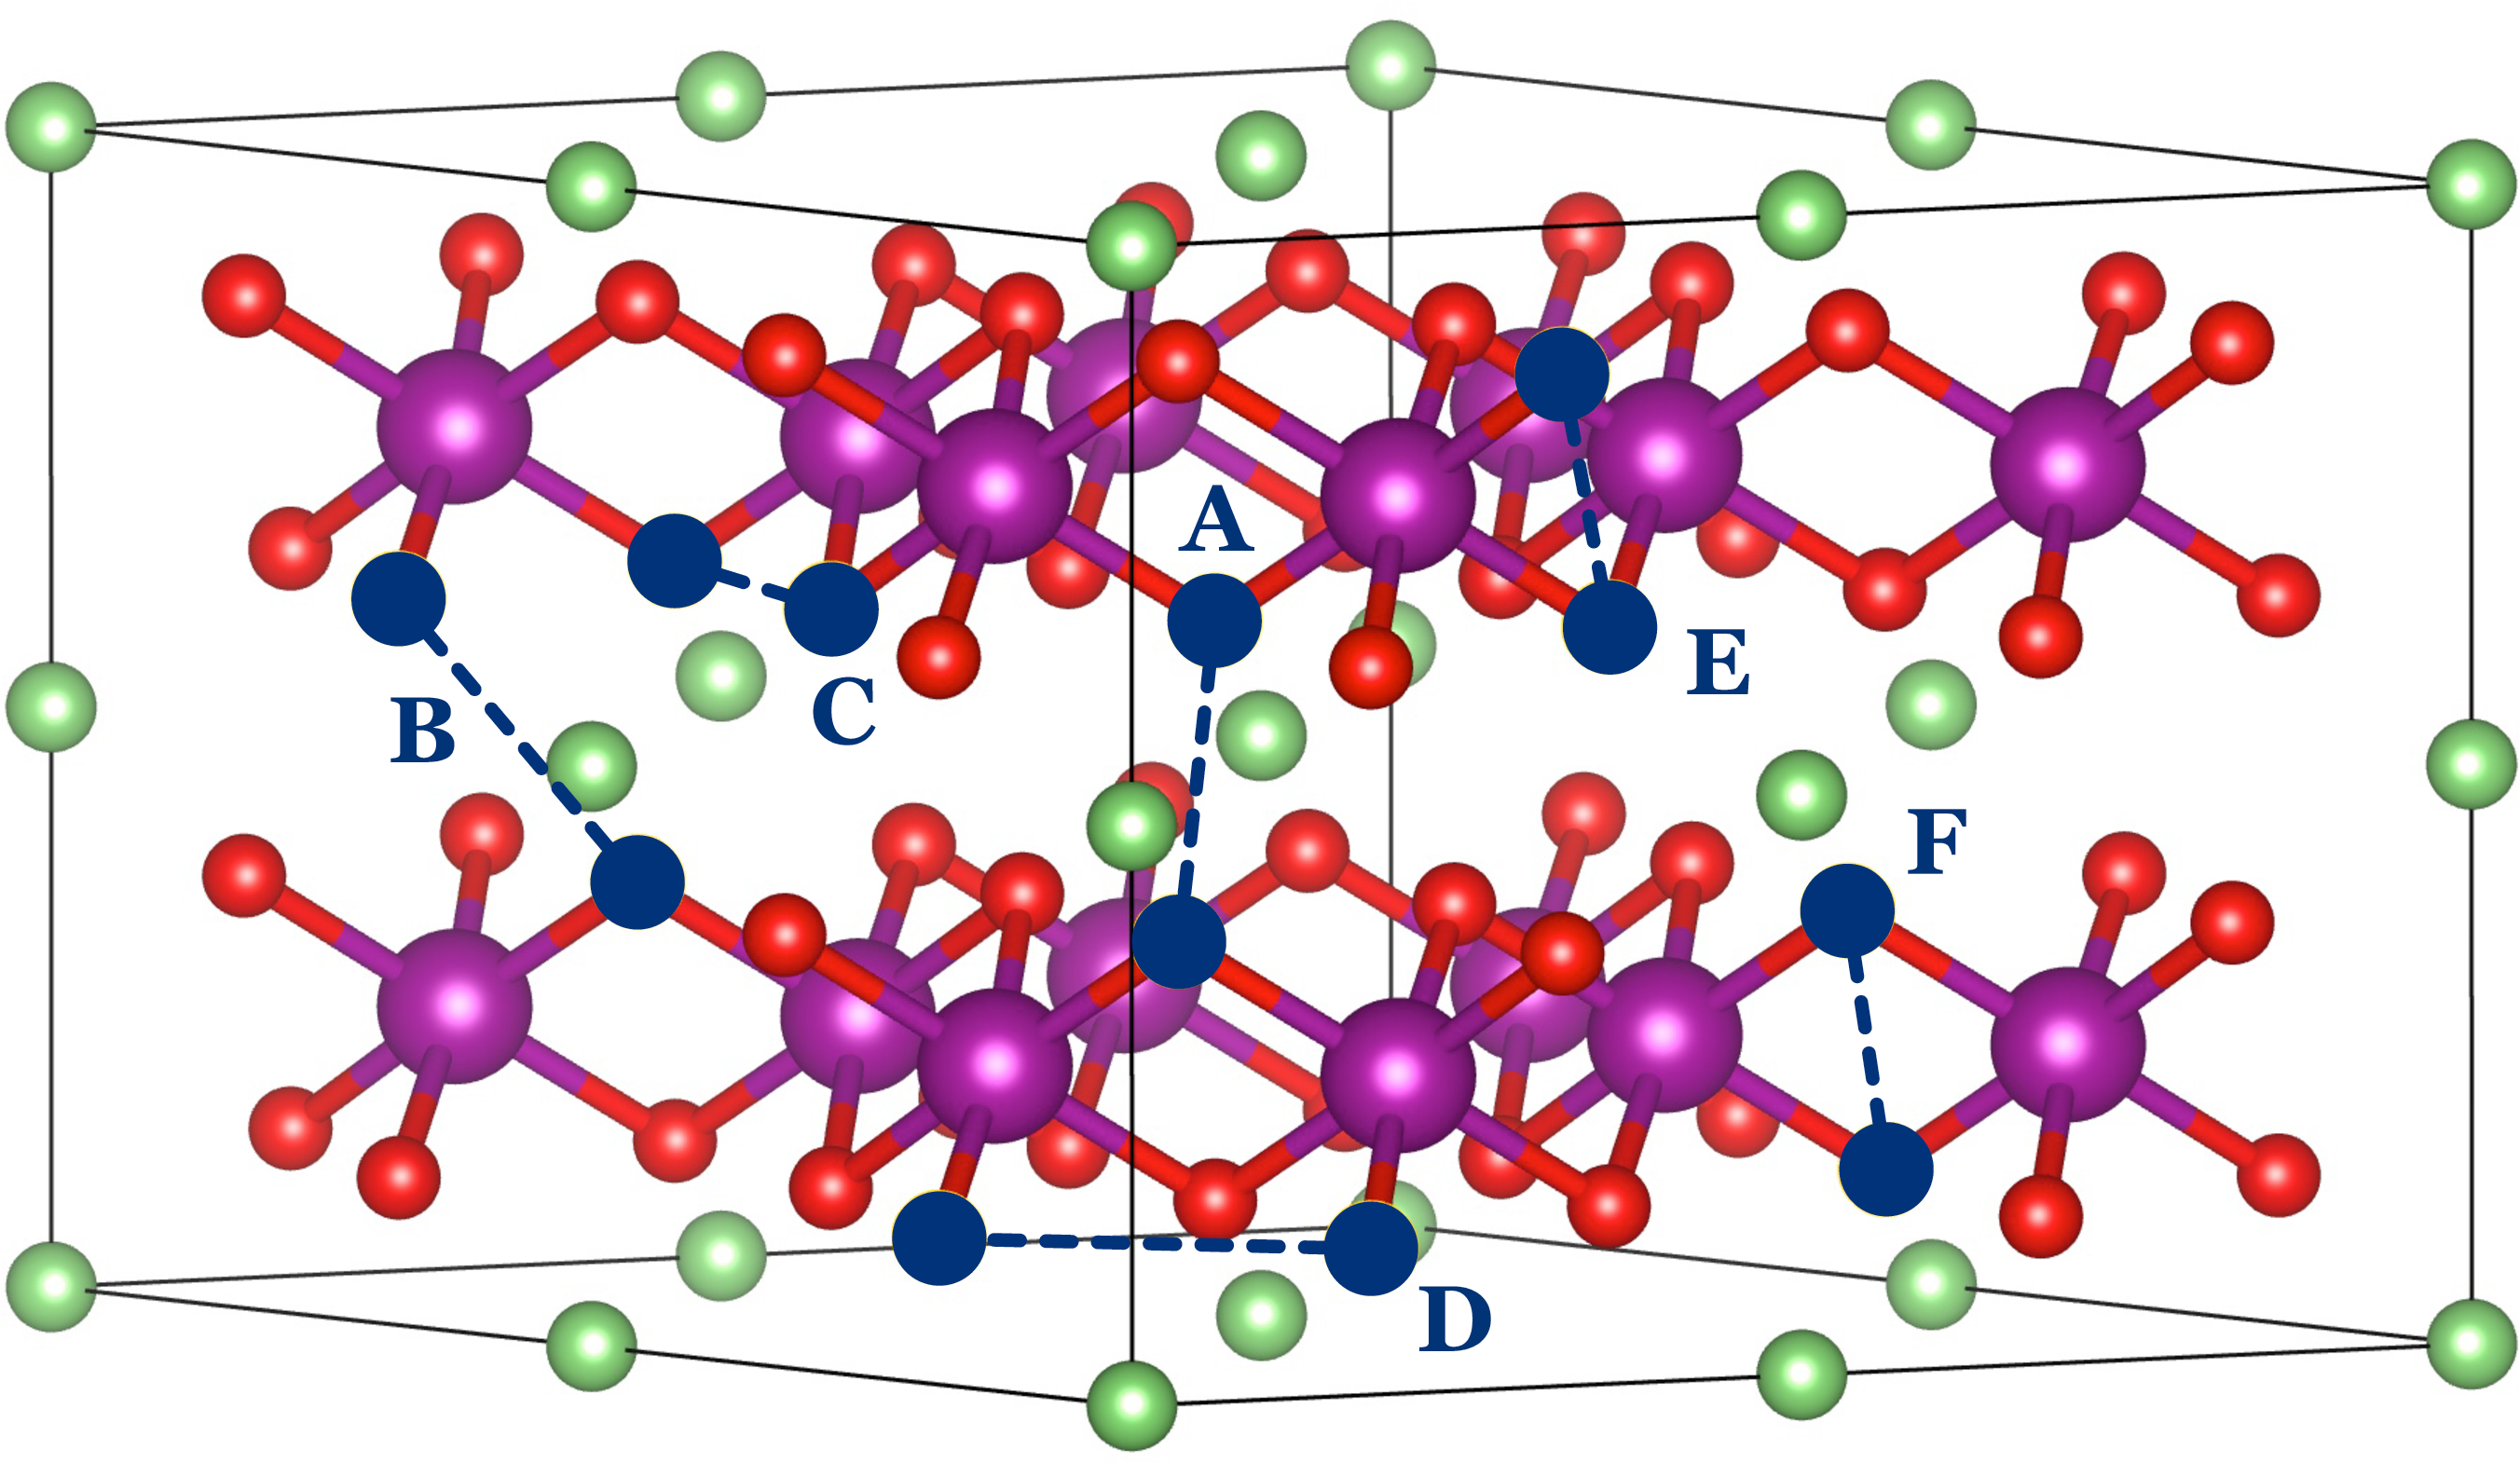
\includegraphics[width=0.6\textwidth]{Figures/batteries/oxygen_dimers.png} 
\caption{Potential oxygen dimers in O1-\ce{Li_{0.5}[Mn, Ir]O3}.} 
\label{batteries:fig-oxygen_dimers}  
\end{figure} 
 
To calculate the chemical reaction energy of the dimer formation, we construct 
a 2$\times$2$\times$2 supercell of the primitive unit cell, for the O1 stacking of 75\% 
charged \ce{Li_{0.5}MnO3} and \ce{Li_{0.5}IrO3} 
(Fig.~\ref{batteries:fig-oxygen_dimers}). In order to consistently study the 
dimer formation, we need to consider all non-equivalent oxygen pairs that have 
the potential to form a dimer for each material. We use the workflow described 
in Section~\ref{automation:sec-dimer} to calculate the reaction energy of all
non-equivalent potential dimers in the structure. In short, all potential oxygen dimers 
in the structure are found using a voronoi decomposition to find the neighbors 
of the various atoms in the unit cell. Once all oxygen dimers have been found, 
we set up a list of all non-equivalent potential dimers based on the
symmetry operations of the structure. In the charged 
\ce{O1-Li_{0.5}MnO3} and O1-\ce{Li_{0.5}IrO3} structures, we find a total of 6 
non-equivalent dimers, shown in Figure~\ref{batteries:fig-oxygen_dimers}. For 
each structure and each potential dimer, we reduce the distance between the 
oxygen atoms in the dimer pair to 1.4~\si{\angstrom} and once again optimize 
all atomic positions as described in the methods section. To make sure the 
interaction between the dimers in the periodic boundary conditions approach of 
VASP is sufficiently small, we have also performed similar calculations in a 
3$\times$3$\times$3 supercell, and found the differences between the reaction energies to be 
smaller than 50~\si{\milli\electronvolt} for all potential 
dimers~\cite{Levi2020}. 
 
\begin{figure}[ht] 
\centering
\captionsetup{width=0.9\linewidth}
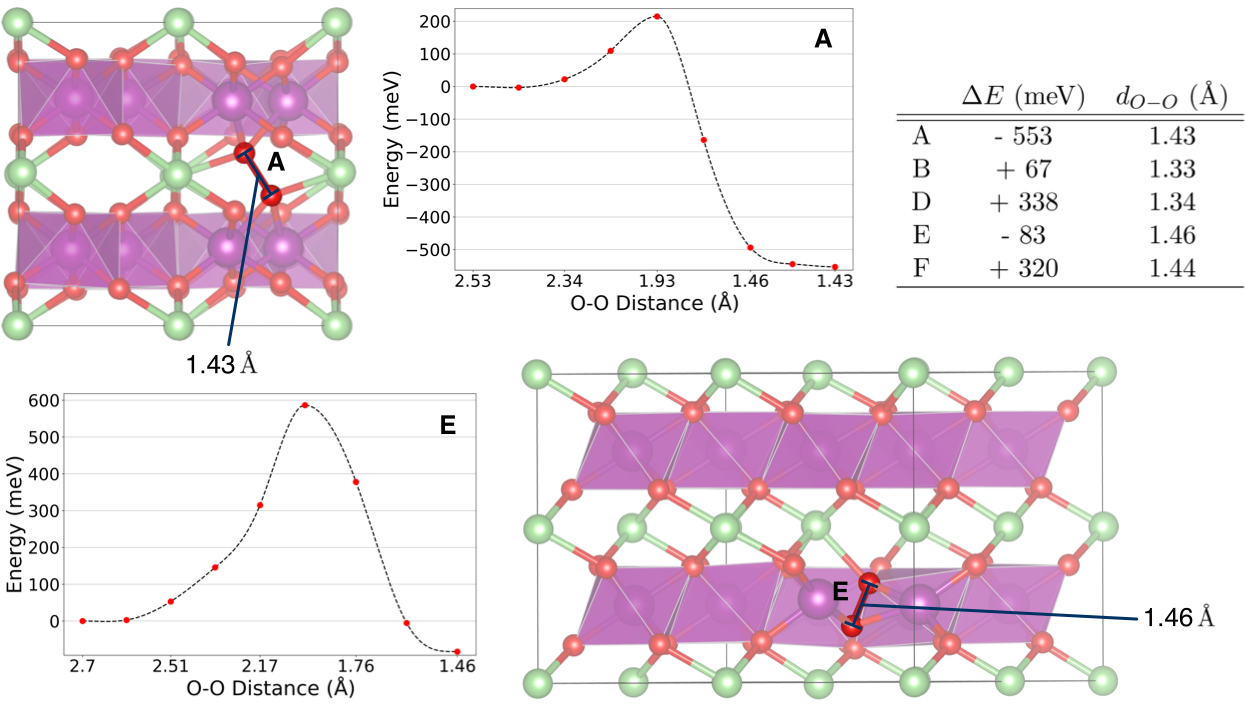
\includegraphics[width=\textwidth]{Figures/batteries/dimer_energetics.png} 
\caption{Reaction energies $\Delta E$, final O-O bond length $d_{O-O}$ and 
kinetic barriers for the dimers in O1-\ce{Li_{0.5}MnO3}. The final geometry 
and kinetic barrier is only shown for dimer \textbf{A} and \textbf{E}, which 
have a negative reaction energy.} 
\label{batteries:fig-Mn_dimers} 
\end{figure} 
 
Figure~\ref{batteries:fig-Mn_dimers} shows the results for the reaction energy 
and final bond length. Even though all perturbed structures 
produce a stable oxygen dimer after optimization, only two dimers have a 
negative reaction energy, which are labelled as \textbf{A} and \textbf{E} 
in Fig.~\ref{batteries:fig-oxygen_dimers}. One dimer (\textbf{C}) results in a 
geometry similar to the formation of the \textbf{E} dimer, with comparable 
energies. The two dimers that have a reduced energy in the final state are 
formed by two oxygen atoms from different layers, with dimer \textbf{A} being 
the most energetically favorable by far. The final structures of both 
dimers are shown in Fig.~\ref{batteries:fig-Mn_dimers}, along with the kinetic barrier, 
calculated using the NEB method. For the \textbf{A} dimer, the kinetic barrier 
is equal to 214~\si{\milli\electronvolt}, which is smaller than the typical 
kinetic barrier for lithium migration in layered 
structures~\cite{VanDerVen2013}. This implies that the formation of the 
\textbf{A} dimer is very likely to occur during the charging process. The 
kinetic barrier for the \textbf{E} dimer is significantly higher at 
584~\si{\milli\electronvolt}, but is by no means insurmountable. Hence, we 
would expect to find both dimers to play a significant role in the structural 
changes that occur for \ce{Li2MnO3} as it is cycled. 
 
In stark contrast with the results of O1-\ce{Li_{0.5}MnO3}, none of the dimer 
optimizations for O1-\ce{Li_{0.5}IrO3} result in a new geometry with a lower 
energy as the unperturbed structure. In fact, out of all the dimers, all but 
one return to the original oxygen framework. The only dimer that is stable 
after optimization has an increased energy of +2.2~\si{\electronvolt}, and is 
hence unlikely to ever be formed in practice. In our view, the enhanced 
stability of the oxygen framework can be in part explained by the reduced 
participation of oxygen in the redox process as the battery is charged, which 
is believed to be the primary driver for dimer formation. 
 
\section{Substitutions} \label{batteries:sec-substitutions} 
 
Based on the discussion from Section~\ref{batteries:sec-lirich}, it is clear 
that the stability of the oxygen lattice plays an important role in 
maintaining the structure of Li-rich cathodes as the battery is cycled. One 
suggested strategy for stabilizing the oxygen framework is the (partial) 
substitution of \ce{Mn^{4+}} by other elements. Based on our results, as well 
as the results of McCalla et al.~\cite{McCalla2015}, \ce{Ir^{4+}} seems like a 
natural choice, as this leads to an improved stability of the structure and 
hence better cycling properties. However, designing a \ce{Ir}-based cathode 
material is not a practical approach due to the weight and price of \ce{Ir}. 
 
Another element that has been suggested in order to improve the cycling 
behaviour of Li-rich materials is \ce{Sn^{4+}}, for several reasons. First, 
the bonding energy of \ce{Sn-O} is higher than that of \ce{Mn-O}, which can 
enhance the structural stability~\cite{Qiao2015}. Second, \ce{Sn^{4+}} does 
not tend to adopt a tetrahedral coordination~\cite{Sathiya2013} and has a much 
larger ionic radius compared to \ce{Mn^{4+}}, implying that the migration of 
\ce{Sn^{4+}} to the \ce{Li} layers is less likely to occur as the battery is 
charged\footnote{Note that the migration path for \ce{Sn^{4+}} does not have 
to pass a tetrahedral site in case the stacking is changed from O3 to O1.}. 
For these reasons, \ce{Sn^{4+}} was chosen as the first element by our 
experimental collaborators from Hasselt University\footnote{Andreas Paulus, 
Marlies van Bael and An Hardy, \href{https://www.uhasselt.be/UH/IMO/Visit-the-groups/Inorganic-and-physical-chemistry-(IPC).html}{Inorganic and Physical Chemistry}, Hasselt University.} to substitute in 
Li-rich NMC samples in an attempt to improve the cycling properties of the 
cathode. 

In this section, I start by briefly discussing their power X-ray diffraction (PXRD) results, as well as 
the energy-dispersive X-ray analysis (EDX) results of our collaborators within EMAT\footnote{Myl\`ene Hendrickx, Olesia 
Karakulina, Artem Abakumov and Joke Hadermann, \href{https://www.uantwerpen.be/en/research-groups/emat/}{Electron Microscopy for Materials 
Science}, Antwerp University.}, as a motivation for the 
calculations we have performed on the solubility of \ce{Sn} in a 
Li-rich/Mn-rich material. Next, I perform a similar analysis as in the 
previous section for investigating the influence of Sn-substitution on the 
stability of the oxygen framework. Finally, I extend this analysis to the 
substitution of several other elements that have the potential to oxidize 
further (\ce{Co}, \ce{V} and \ce{Mo}), in order to investigate if they have a 
stabilizing effect similar to that of \ce{Ir}.  

\resultsubsection{Thermodynamic Stability of Sn substitution \label{batteries:sec-Sn_stability}}{https://github.com/mbercx/phd-thesis/tree/master/jupyter/batteries\#thermodynamic-stability-of-sn-substitution}{sn_stability}
 
Although the increased ionic radius of \ce{Sn^{4+}} compared to \ce{Mn^{4+}} 
is believed to inhibit its migration into the Li-layer, it can potentially 
also lead to a reduced solubility of \ce{Sn} in the NMC structure. In order to 
investigate the solubility of Sn in Li-rich NMC, several samples with 
increased Sn-substitution were prepared for a Li-rich/Mn-rich NMC structure, 
leading to stoichiometries \ce{Li_{1.2}Ni_{0.13}Co_{0.13}Mn_{0.54-x}Sn_xO2} 
for $x  \approx 0, 0.027, 0.054, 0.108 \textrm{ and } 0.54$. Looking at the 
change in the powder XRD pattern of Sn-substituted NMC samples in 
Fig.~\ref{batteries:fig-Sn_experiment}~(a), a second phase appears as the 
amount of Sn is increased, starting from $x = 0.054$. This phase becomes dominant for $x=0.54$ and was 
identified as \ce{Li2SnO3} based on an indexation of the PXRD results. 
The EDX results for a particle with $x=0.108$ 
(Fig.~\ref{batteries:fig-Sn_experiment}) indicate that the exsolution of this 
Sn-rich phase already occurs at lower levels of Sn-substitution. 
 
\begin{figure}[ht] 
    \centering
    \captionsetup{width=0.92\linewidth}
    \begin{subfigure}[t]{0.65\textwidth} 
        \centering 
        \includegraphics[width=\textwidth]{./figures/batteries/xrd_Sn_substitution.png} 
        \caption{} 
    \end{subfigure}% 
    ~  
    \begin{subfigure}[t]{0.34\textwidth} 
        \centering 
        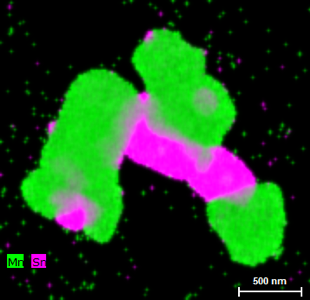
\includegraphics[width=0.9\textwidth]{./figures/batteries/edx_Sn_substitution.png} 
        \caption{} 
    \end{subfigure} 
    \caption{(a) PXRD patterns of 
\ce{Li_{1.2}Ni_{0.13}Co_{0.13}Mn_{0.54-x}Sn_xO2} for increasing values of 
Sn-substitution $x$. (b) Mixed (Mn, Sn) elemental EDX map of representative 
LNMCS20 (x=0.108) particles. Courtesy of Andreas Paulus (a) and Myl\`ene 
Hendrickx (b).} 
    \label{batteries:fig-Sn_experiment} 
\end{figure} 
 
To determine the \ce{Sn} solubility computationally, we investigate the 
thermodynamic stability of Sn-substituted structures versus their 
decomposition into an Mn-rich and Sn-rich phase. However, some approximations 
must be made in order to make the problem computationally feasible. First, 
including four different elements (\ce{Ni}, \ce{Mn}, \ce{Co} and \ce{Sn}) in 
our calculations would make both the number of configurations and reaction 
products prohibitively large, so we limit our study to the solubility of 
\ce{Sn} in \ce{Li_{1.2}Mn_{0.8}O2}. Considering the similar ionic radii of 
\ce{Mn^{4+}}, \ce{Co^{4+}} and \ce{Ni^{4+}}, this should not affect our 
conclusion significantly. Using this approximation, we first consider the 
following exsolution reaction: 
\begin{equation} 
 \ce{Li_{1.2}Mn_{0.8-x}Sn_xO2} \rightarrow  \left( 1 - \frac{x}{0.8} \right) 
\ce{Li_{1.2}Mn_{0.8}O2} +  \frac{x}{0.8} \ce{Li_{1.2}Sn_{0.8}O2}  
\end{equation} 
The PXRD results indicate, however, that the final Sn-rich phase most likely 
corresponds to \ce{Li2SnO3} and, to a lesser extent, \ce{SnO}. This means that 
the following exsolution reaction is more probable: 
\begin{equation} \label{batteries:eq-exsolution} 
 \ce{Li_{1.2}Mn_{0.8-x}Sn_xO2} \rightarrow  \left( 1 - \frac{x}{0.8} \right) 
\ce{Li_{1.2}Mn_{0.8}O2} +  \frac{x}{0.8} \left[  0.6 \cdot \ce{Li2SnO3} + 0.2 
\cdot \ce{SnO} \right] 
\end{equation} 
 
Finally, there is another restriction to which our structures should adhere: 
based on the HAADF-STEM results for several of the Sn-substituted samples, the 
honeycomb ordering of the \ce{Li}-TM/\ce{Sn} cations is largely 
maintained\footnote{Note that as the ratio of \ce{Li} over TM/\ce{Sn} elements 
is smaller than 2, it is no longer possible to have a complete honeycomb 
ordering in the  \ce{Li}-TM/\ce{Sn} layer, as was the case for \ce{Li2MnO3}.}. 
This leads to the following construction of the \ce{Li_{1.2}Mn_{0.8}O2} 
structures:  
\begin{itemize} 
\item Start from the pristine primitive structure of O3-\ce{Li2MnO3}, with 
space group $C2/m$. 
\item Replace the \ce{Li} in the \ce{Li}/\ce{Mn} layer by a placeholder 
element, e.g. \ce{Lr}. This is just to keep track of which sites correspond to 
the \ce{Li} sites in the honeycomb layer. 
\item Make a 2$\times$2$\times$2 supercell. This size is chosen to get as close as possible 
to the experimental composition of \ce{Li}, without having to consider a unit 
cell size that is prohibitively large. 
\item Use the \texttt{Cathode.get\_cation\_configurations()} method to 
generate honeycomb-like structures by substituting the \ce{Lr} by \ce{Li} and 
\ce{Mn}, restricting the \ce{Li} concentration of the final configurations to 
closely match that of the experimental samples. 
\end{itemize} 
Because of the restrictions of the honeycomb pattern and \ce{Li} 
concentration, this method only results in 5 configurations, each with a 
composition that closely matches the experimental one: 
\ce{Li_{1.2083}Mn_{0.7917}O2} $\approx$ \ce{Li_{1.21}Mn_{0.79}O2}. To generate 
the \ce{Sn}-substituted structures, we consider each of the \ce{Mn} 
configurations, and once again use the 
\texttt{Cathode.get\_cation\_configurations()} method, this time partially 
substituting the \ce{Mn} elements by \ce{Sn}. For a single \ce{Sn} 
substitution in the supercell ($x = 0.042$), there are 47 possible 
\ce{Li}-\ce{Mn}-\ce{Sn}, which is still a manageable amount to handle with our 
configuration workflow. However, increasing the \ce{Sn} content further leads 
to 361/1867/7202 configurations for $x = 0.083/0.125/0.167$ respectively. 
Optimizing the geometry of all these configurations is clearly not possible, 
so we have to limit the number of configurations to a more manageable number.  
 
Before analysing the reaction in Eq.~\ref{batteries:eq-exsolution}, it is 
important to confirm that the \ce{Sn}-rich phase is more likely to be a 
combination of \ce{Li2SnO3} and \ce{SnO} than \ce{Li_{1.2}Sn_{0.8}O2}. For 
this purpose, we first generate all \ce{Li}-\ce{Sn} configurations of 
\ce{Li_{1.2}Sn_{0.8}O2}, similar to the procedure described in the previous 
paragraph. Next, we optimize the geometry and calculate the energy of all 5 
configurations, along with the energies of \ce{Li2SnO3} and \ce{SnO}. Note 
that, similar to the \ce{Li}-rich \ce{Mn} structure, the composition of the 
configurations is closer to \ce{Li_{1.2083}Sn_{0.7917}O2}.This means that the 
effective decomposition reaction of interest is: 
\begin{equation} \label{batteries:eq-Sn-decomposition} 
\ce{Li_{1.2083}Sn_{0.7917}O2} \rightarrow  A  \cdot \ce{Li2SnO3} + B \cdot 
\ce{SnO}, 
\end{equation} 
where $A \approx 0.604$ and $B = 0.1875$. The corresponding formation energy 
is: 
\begin{equation} 
E_f = E(\ce{Li_{1.2083}Sn_{0.7917}O2}) - A \cdot E(\ce{Li2SnO3}) - B \cdot 
E(\ce{SnO}), 
\end{equation} 
which for the lowest energy configuration of \ce{Li_{1.2083}Sn_{0.7917}O2} is 
equal to 459~\si{\milli\electronvolt}. Considering the significantly larger 
energy of \ce{Li_{1.2083}Sn_{0.7917}O2} compared to \ce{Li2SnO3} and \ce{SnO}, 
it is reasonable to suggest that the \ce{Sn}-rich phase corresponds more 
closely to a combination of these end products. 
 
Finally, the exsolution reaction becomes: 
\begin{equation} \label{batteries:eq-exsolution_final} 
 \ce{Li_{1.21}Mn_{0.79-x}Sn_xO2} \rightarrow  \left( 1 - \frac{x}{0.79} 
\right) \ce{Li_{1.21}Mn_{0.79}O2} +  \frac{x}{0.79} \left[  0.604 \cdot 
\ce{Li2SnO3} + 0.1875 \cdot \ce{SnO} \right], 
\end{equation} 
with formation energy 
\begin{align} \label{batteries:eq-exsolution_final_formation} 
 E_f(x) = E(\ce{Li_{1.21}Mn_{0.79-x}Sn_xO2}) -  \left( 1 - \frac{x}{0.79} 
\right) E(\ce{Li_{1.21}Mn_{0.79}O2}) \nonumber \\ -  \frac{x}{0.79} \left[  0.604 \cdot 
E(\ce{Li2SnO3}) + 0.1875 \cdot E(\ce{SnO}) \right], 
\end{align} 
 
%However, instead of choosing the configurations randomly, it is better to 
% first rank the configurations by their electrostatic energy~\cite{Seo2016}, 
% calculated using the Ewald summation method. 
 
\begin{figure}[ht] 
\centering 
\captionsetup{width=0.9\linewidth}
\includegraphics[width=0.7\textwidth]{figures/batteries/Sn_mixing_energy.png} 
\caption{Calculated formation energies using 
Eq.~(\ref{batteries:eq-exsolution_final_formation}) for all configurations 
with $x = \{i/24|i=1,2,3,4,5\}$.} 
\label{batteries:fig-Sn_mixing} 
\end{figure} 
 
Figure~\ref{batteries:fig-Sn_mixing} shows the calculated formation energies 
for 40 configurations of the Sn substituted structures for each $x = 
\{i/24|i=1,2,3,4,5\}$, compared to their decomposition in 
\ce{Li_{1.21}Mn_{0.79}O2}, \ce{Li2SnO3} and \ce{SnO}. For the lowest Sn 
concentration, x = 0.042, the formation energy of the lowest energy 
configuration is only +6.5 meV/atom. This structure can 
reasonably be considered as metastable~\cite{Sun2016} and as such the 
formation of a single phase is feasible at low Sn concentrations. However, as 
the Sn-concentration $x$ is increased, the \ce{Li_{1.2}Mn_{0.8-x}Sn_xO2} 
configurations become more unstable, increasing the likelihood of a 
decomposition in \ce{Li_{1.2}Mn_{0.8}O2}, \ce{Li2SnO3} and \ce{SnO} phases, as 
observed in the PXRD results for the high Sn concentration samples. Note that 
if the Sn substituted orderings are generated randomly, i.e. without 
respecting the honeycomb pattern, the energies are significantly higher 
compared to the honeycomb structures at each Sn concentration. This matches 
the preservation of the honeycomb ordering for the Sn substituted structure 
found for the HAADF-STEM results. 
 
\resultsubsection{Influence of \ce{Mn^{4+}} substitution on oxygen stability \label{batteries:sec-dimer_substitution}}{https://github.com/mbercx/phd-thesis/tree/master/jupyter/batteries\#influence-of-mn4-substitution-on-oxygen-stability}{substitutions} 

The next question is whether the stability of the oxygen framework of 
\ce{Li2MnO3} can be improved by a local substitution of \ce{Mn^{4+}} by \ce{Sn^{4+}}. In order 
to make a fair comparison with the results presented in 
Sections~\ref{batteries:sec-oxidation} and \ref{batteries:sec-dimer}, we start 
from the 2$\times$2$\times$2 supercell of the charged O1-\ce{Li_{0.5}MnO3} structure. Based 
on the results of the previous section, only a limited amount of \ce{Sn} can 
be substituted in~\ce{Li2MnO3} before we expect the cathode to separate in several 
phases, and hence we simply substitute a single \ce{Mn} atom by \ce{Sn}. In 
light of the discussion of Section~\ref{batteries:sec-lirich},  however, we 
would not expect \ce{Sn} to be very effective in stabilizing the oxygen 
framework, as it is unable to oxidize beyond +4. Hence, we expand our search 
of suitable substitutions to \ce{V} and \ce{Mo}, two elements that permit 
higher states of oxidation and have shown promise in \ce{Li}-rich 
materials~\cite{Ma2014, Xiao2012}. Moreover, in order to study the influence of 
the exchange-correlation functional, we make a comparison between the \dft{PBEU}{} results and the 
recently introduced \dft{SCAN}{}. 
In contrast to PBE+U, SCAN does not rely on an element-dependent parameter, 
so it would be interesting to see if it produces a similar trend for the 
barrier of the various substituted elements.
This discussion, however, is left for the end of this section.
 
\begin{table}[ht] 
\centering 
\captionsetup{width=0.9\linewidth}
\renewcommand{\arraystretch}{1.3} 
\caption{Calculated absolute values of the magnetic moments for the discharged 
and charged for the \ce{Sn}/\ce{V}/\ce{Mo}-substituted structures, all 
expressed in Bohr magnetons $\mu_B$. For the oxygen, we make a distinction between the 
neighbours of the substituted element \ce{O_n} and other oxygen elements in 
the unit cell \ce{O_o}.} 
\label{batteries:tab-substitution_magmoms} 
\begin{tabular}{c c c c c c c} 
 & & \multicolumn{2}{c}{PBE+U} & & 
\multicolumn{2}{c}{SCAN}\\\cline{3-4}\cline{6-7} 
 & & discharged & charged & & discharged & charged \\\hline 
\multirow{3}{*}{Sn} & \multicolumn{1}{|c}{$|\mu|$ (\ce{Sn})} & 0.018 & 0.045 & 
& 0.017 & 0.064 \\ 
 & \multicolumn{1}{|c}{$|\mu|$ (\ce{O_n})} & 0.021 & 0.434 & & 0.020 & 0.355 
\\ 
 & \multicolumn{1}{|c}{$|\mu|$ (\ce{O_o})} & 0.000 & 0.463 & & 0.000 & 0.333 
\\\hline 
\multirow{3}{*}{V} & \multicolumn{1}{|c}{$|\mu|$ (\ce{V})} & 0.953 & 0.270 & & 
0.875 & 0.260 \\ 
 & \multicolumn{1}{|c}{$|\mu|$ (\ce{O_n})} & 0.012 & 0.329 & & 0.032 & 0.219 
\\ 
 & \multicolumn{1}{|c}{$|\mu|$ (\ce{O_o})} & 0.000 & 0.459 & & 0.000 & 0.322 
\\\hline 
\multirow{3}{*}{Mo} & \multicolumn{1}{|c}{$|\mu|$ (\ce{Mo})} & 1.792 & 0.172 & 
& 1.293 & 0.110 \\ 
 & \multicolumn{1}{|c}{$|\mu|$ (\ce{O_n})} & 0.028 & 0.208 & & 0.001 & 0.128 
\\ 
 & \multicolumn{1}{|c}{$|\mu|$ (\ce{O_o})} & 0.001 & 0.446 & & 0.000 & 0.310 
\\\hline 
\end{tabular} 
\end{table} 
 
Table~\ref{batteries:tab-substitution_magmoms} contains the magnetic moments 
and Figure~\ref{batteries:fig-substitution_pdos_pbeu} shows the projected 
density of states near the Fermi level for the 
\ce{Sn}/\ce{V}/\ce{Mo}-substituted structures, both in the discharged and 
charged state. For \ce{Sn}, there are practically no states in near the Fermi 
level, which is not surprising considering that in a +4 oxidation state, Sn 
has donated its 5$s$ and 5$p$ valence electrons to the surrounding oxygen. 
This is also clear from the magnetic moments, which are close to zero for 
\ce{Sn} in both states of charge. Because of this inability of \ce{Sn} to 
oxidize further, the oxygen redox is similar to that of undoped \ce{Li2MnO3}. 
In light of this, it is unsurprising that the kinetic barrier for the A dimer 
in the 75\% charged Sn-doped structure is similar, even when one of the oxygen atoms neighbours the substituted 
\ce{Sn} (Fig.~\ref{batteries:fig-substitution_dimers}). 

\pagebreak[5] For \ce{V} and \ce{Mo}, the magnetic moments and projected density of states 
are also in the line of expectations. Both substituted elements show a clear 
change in their magnetic moment, indicating that they have oxidized further 
as the battery is charged. The neighbouring oxygens \ce{O_n} also have a 
significantly lower magnetic moments compared to other oxygen atoms \ce{O_o} 
for the charged structure, confirming the decreased oxidation of the oxygen 
framework around the substituted element. Looking at the projected density of 
states in Fig.~\ref{batteries:fig-substitution_pdos_pbeu}, the \ce{V} and 
\ce{Mo} states are both right below the Fermi level, basically corresponding 
to donor levels in the band gap of the discharged \ce{Li2MnO3} structure. As 
\ce{Li} is removed from the structure, these states will be the first to be 
depopulated, which matches well with the picture provided by the magnetic 
moments. 
 
\begin{figure}[ht] 
\centering 
\captionsetup{width=0.9\linewidth}
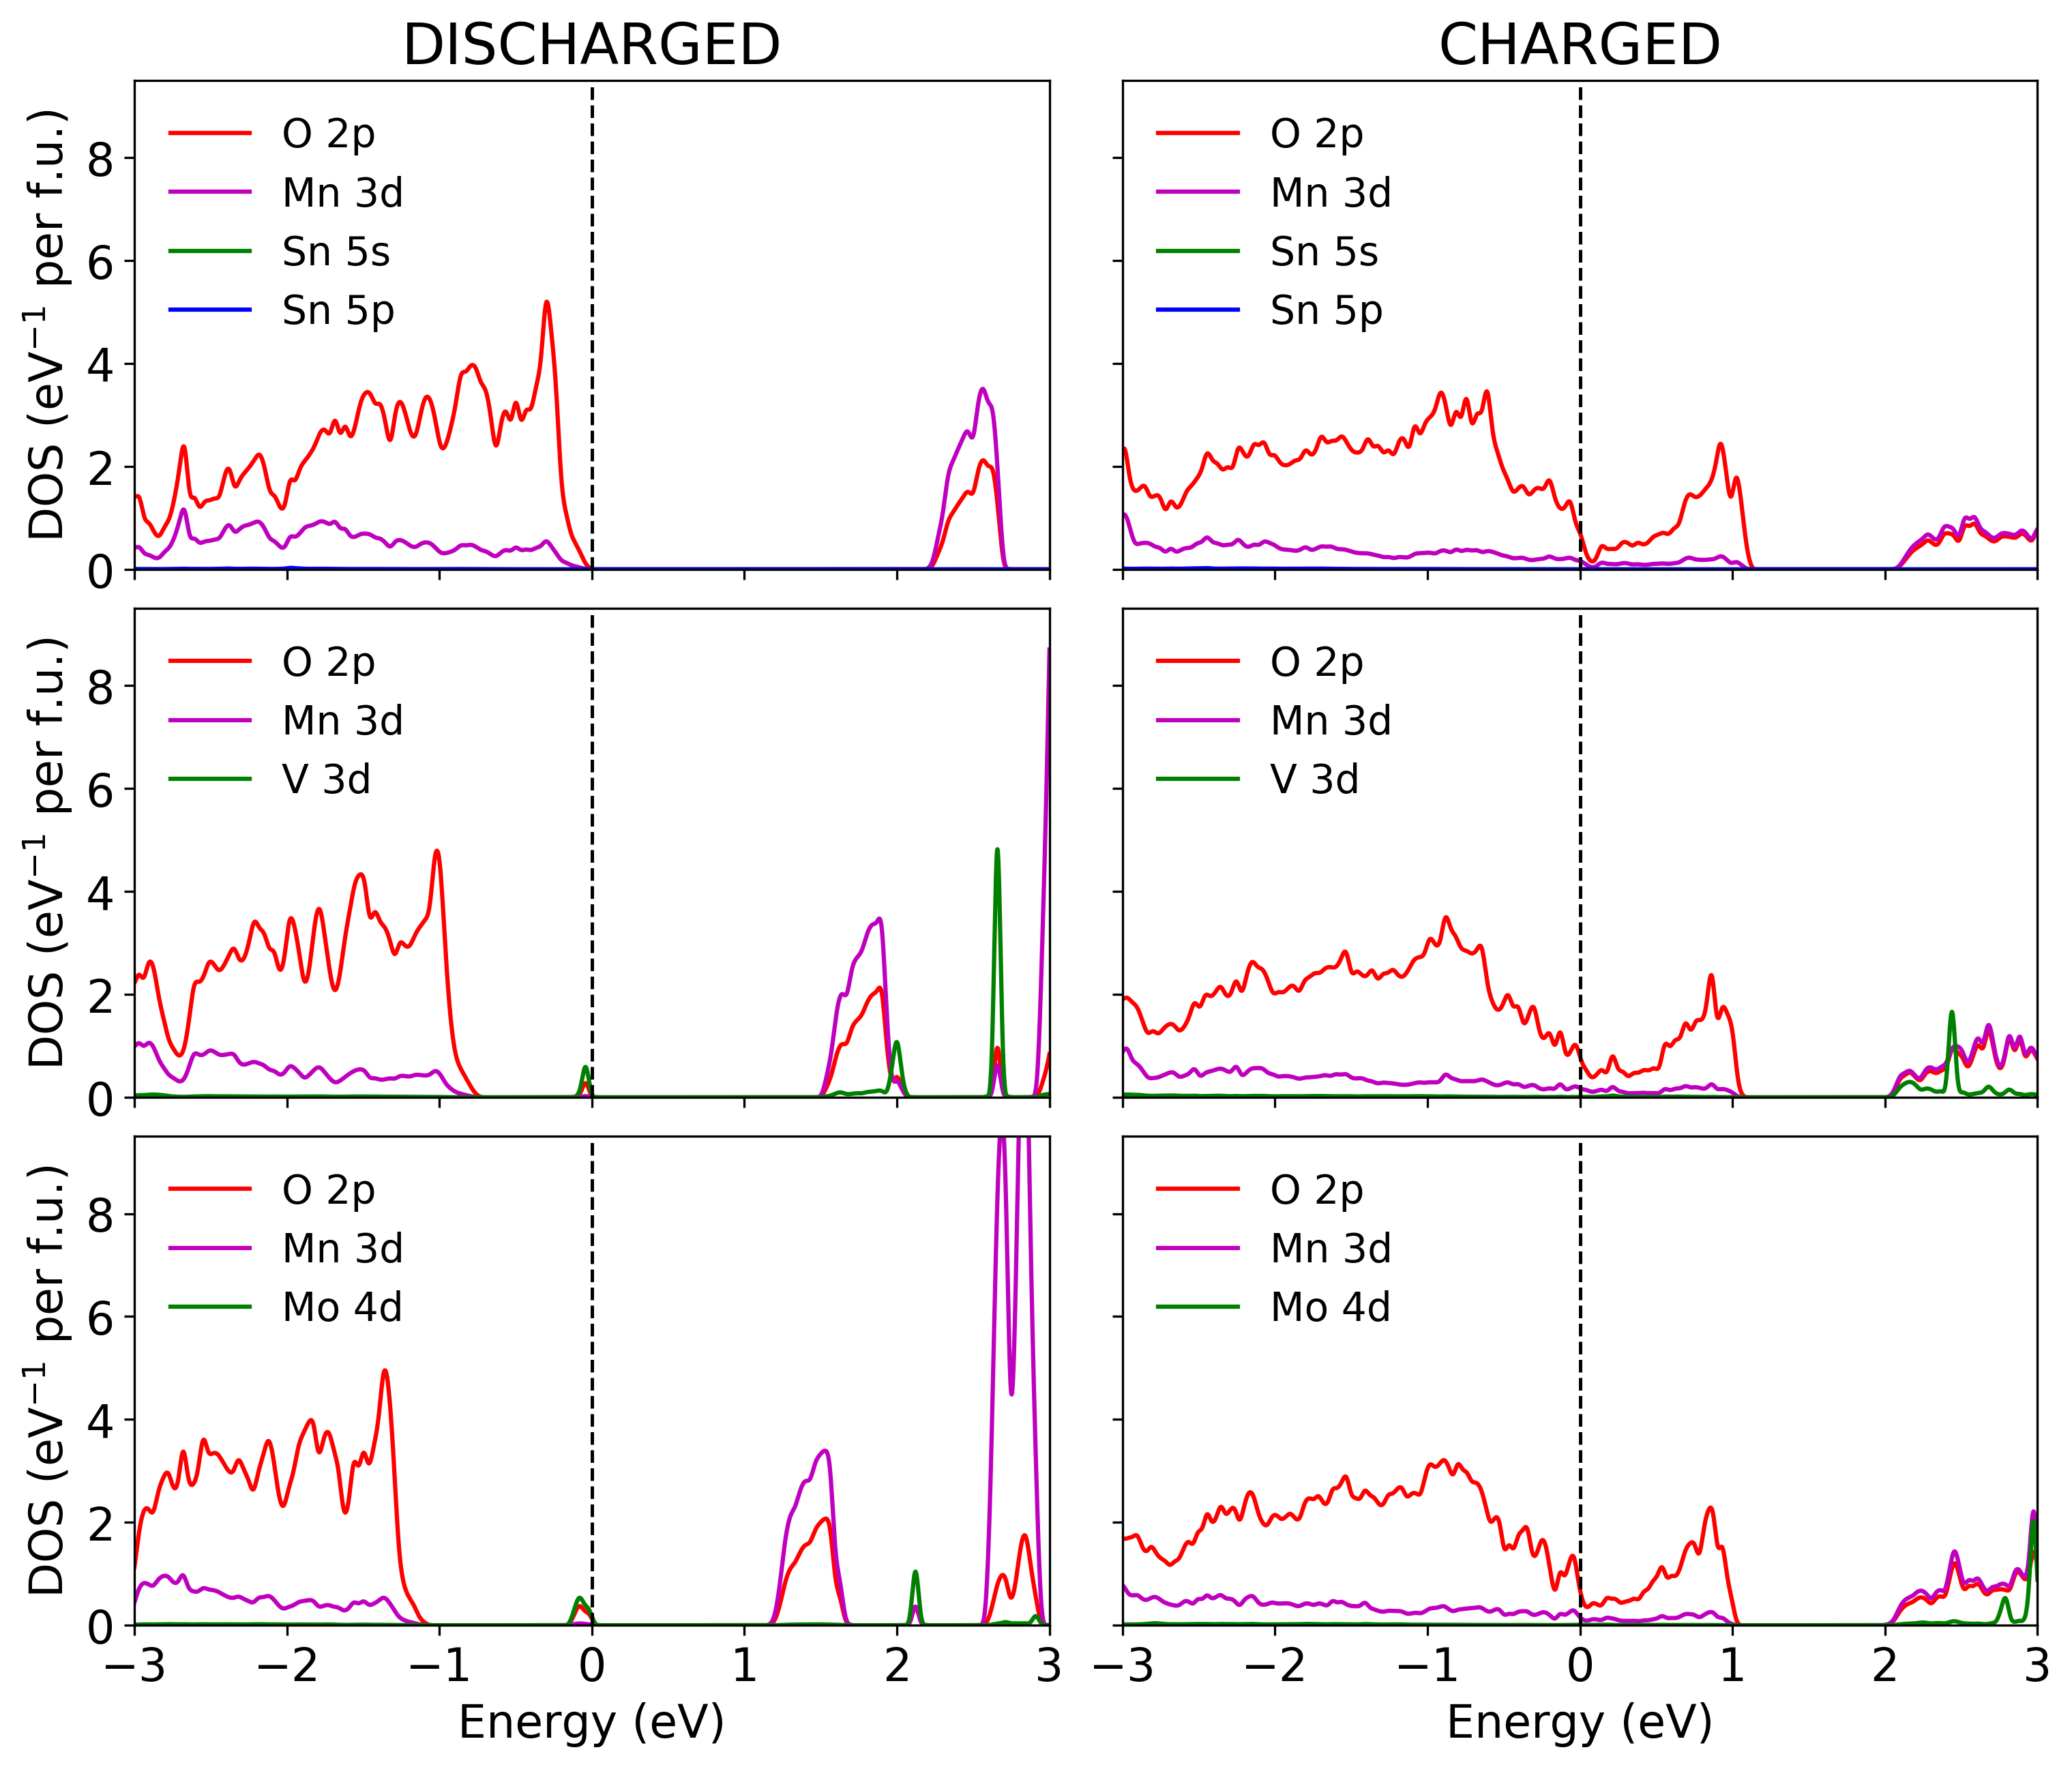
\includegraphics[width=\textwidth]{figures/batteries/substitution_pdos_pbeu.png} 
\caption{Projected density of states for the discharged (left) and charged 
(right) structures, for the 2$\times$2$\times$2 supercell of \ce{Li2MnO3} with a single 
substitution of \ce{Sn}, \ce{V} and \ce{Mo}.} 
\label{batteries:fig-substitution_pdos_pbeu} 
\end{figure} 

However, in contrast to \ce{Ir}, the increased propensity of \ce{V} and 
\ce{Mo} to oxidize does not seem to increase the stability of the surrounding 
oxygen framework. The kinetic barriers for the formation of the \textbf{A} 
dimer, shown in Fig.~\ref{batteries:fig-substitution_dimers}, is easily 
surmountable for both elements, and is in fact even lower compared to that of 
\ce{Li2MnO3}. Considering this, it would appear that neither the substitution 
of \ce{V} nor \ce{Mo} improves the stability of the oxygen framework, despite 
the fact that they are more likely to oxidize before the oxygen.  
 
\newpage
\begin{figure}[ht] 
\centering 
\captionsetup{width=0.9\linewidth}
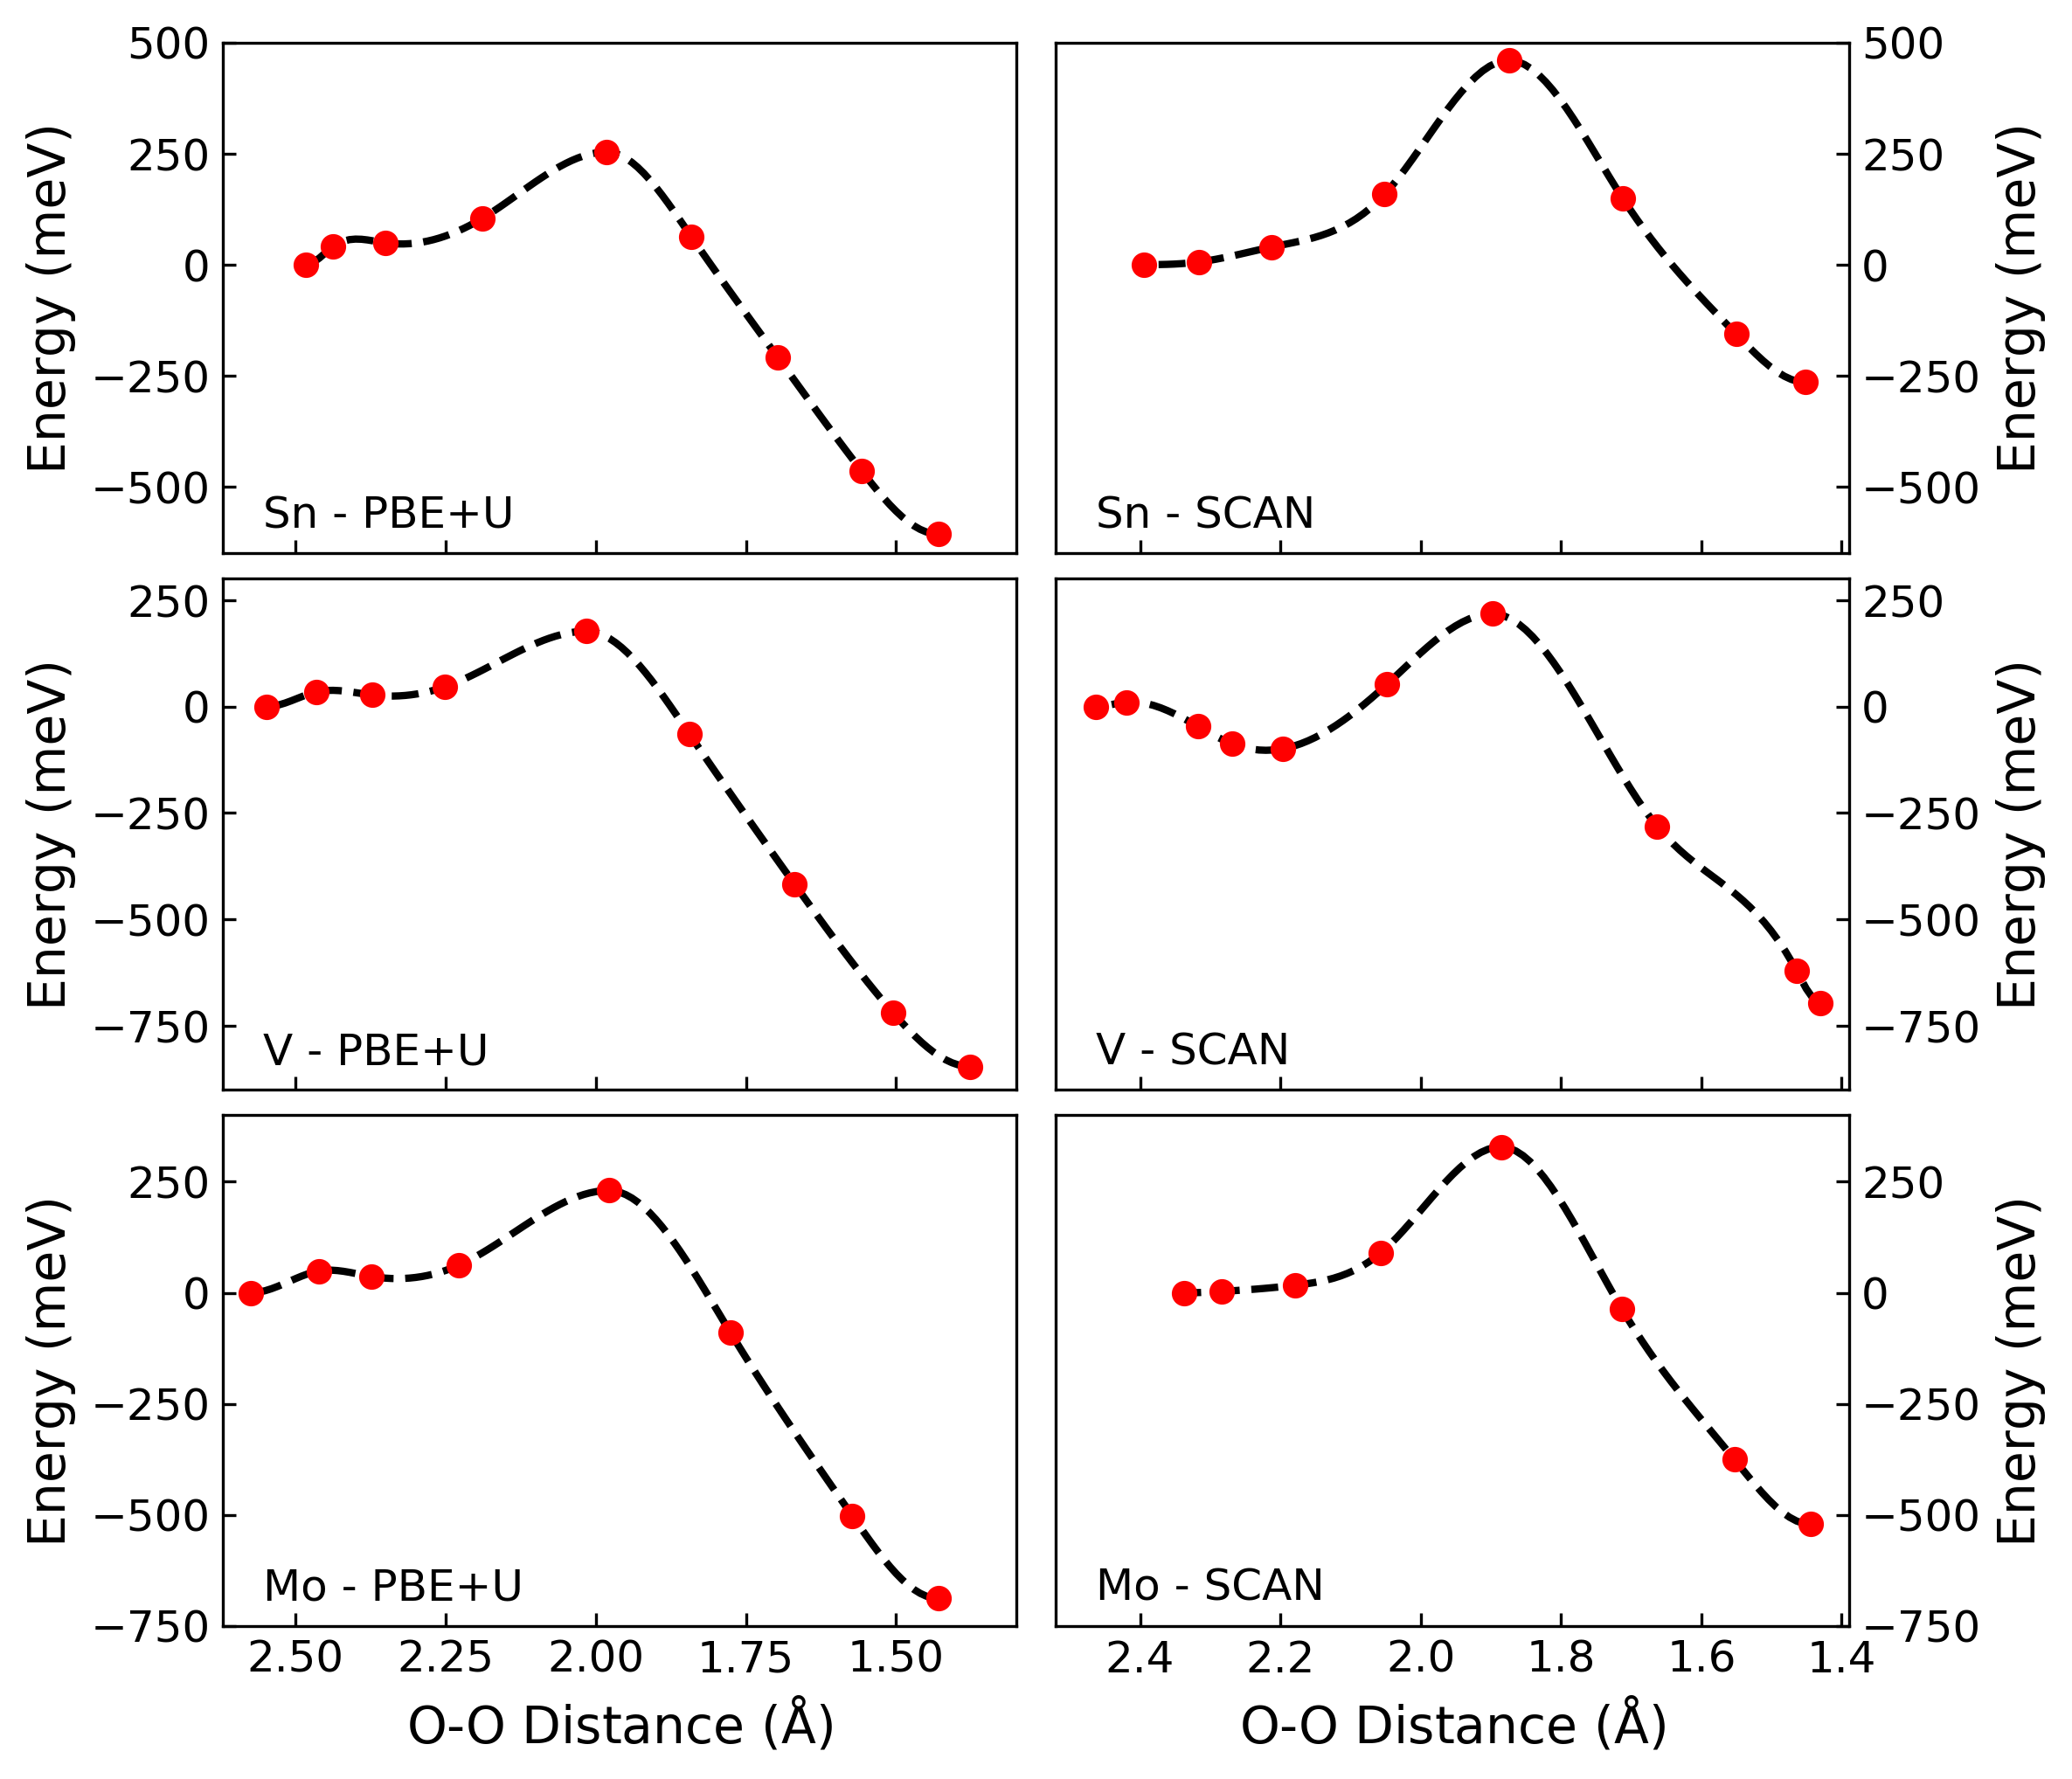
\includegraphics[width=0.85\textwidth]{figures/batteries/substitution_dimers.png} 
\caption{Kinetic barriers for the dimerization of oxygen neighbouring \ce{Sn}, 
\ce{V} and \ce{Mo}, both for the PBE+U and SCAN functional.} 
\label{batteries:fig-substitution_dimers} 
\end{figure} 
 
Finally, we have also performed all of the calculations in this section with 
the recently published \dft{SCAN}{}, in order to compare the results with 
those of \dft{PBEU}{}. As SCAN does not rely on specifying a parameter for each 
transition metal that can influence the oxidation state of the element, this 
provides an unbiased set of data to compare with. Looking at the magnetic 
moments in Table~\ref{batteries:tab-substitution_magmoms}, the discussion from 
the previous paragraphs remains largely intact. However, the magnetic moments 
on the oxygen atoms is decidedly lower compared to the PBE+U results. One 
could argue that this indicates that our choice of Hubbard-U correction might 
have excessively localized the electrons around the transition metals, but a 
similar reduction in magnetic moments is found for the oxygen neighbouring 
\ce{Sn}, for which we have applied no Hubbard-U correction. Moreover, our 
chosen U value for \ce{Mn} has been carefully benchmarked versus our previous 
results for HSE06, which has demonstrated a good ability\footnote{Note that by 
tuning the fraction of exact exchange, it is possible to improve the accuracy 
of the HSE functional further, but \dft{HSE06}{} (a = 0.25) does a fairly good job of 
reproducing experimental results.} for correcting the self-interaction error for 
battery cathodes~\cite{Seo2015}. Looking at the kinetic barriers in 
Fig.~\ref{batteries:fig-substitution_dimers}, SCAN predicts a slightly 
increased barrier for each of the substituted elements, which could be linked 
to the reduced magnetic moment on \textit{all} oxygen atoms. Even this 
increased barrier is still relatively low, however, and hence not much of our 
analysis would if we would base it on the SCAN results. 

\section{Polyborane solid electrolytes} \label{batteries:sec-solid_electrolyte}

Many of the current safety issues that plague Li-ion batteries, such as thermal runaway~\cite{Wang2012} and electrolyte decomposition~\cite{Lisbona2011}, are related to the use of a flammable liquid electrolyte~\cite{Liu2018, Ouyang2019}. To prevent hazardous incidents, complex packaging design is required at the cell, module and pack level~\cite{Dougthy2012} which increases the dead weight of the battery, reducing the energy density. A promising strategy for dealing with these issues is replacing the liquid electrolyte by a solid state ionic conductor. Besides improving the safety, solid state electrolytes also offer improved stability, which significantly increases the lifetime of the battery~\cite{Mauger2019}. Moreover, the electrochemical window of the solid electrolyte is typically larger, which allows for larger operating voltages~\cite{Li2014} and hence significant increases in the energy density. Finally, a solid electrolyte could also enable the development of Li-metal and Li-air batteries, as well as the miniaturization~\cite{Bates2000, Um2017} and three dimensional battery architectures~\cite{Long2004, Pearse2018}. 

A good solid electrolyte must demonstrate a high ionic conductivity and negligible electronic conductivitity at the range of lithium activity and operating temperature of the battery~\cite{Knauth2009}. Other important properties include the chemical stability versus reactions at the electrode interfaces, and good mechanical properties in order to accomodate for the change in volume of the electrodes during the cycling of the battery~\cite{Koerver2018}. Different classes being considered as solid electrolytes include perovskite (e.g. LLTO~\cite{Inaguma1993}), NASICON (e.g. \ce{Na_{1+x}Zr_2Si_xP_{3-x}O_{12}} ($0 \leq x \leq 3$)~\cite{Hagman1968}) and garnet types (e.g. \ce{Li7La3Zr2O12} \cite{Murugan2007}). For a recent overview, we refer the reader to the review papar of Zheng et al.~\cite{Zheng2018}.

Here I present my contribution to the investigation of the theoretical principles behind the superionic conductivity of polyborane salts, a class of materials that has recently demonstrated significant potential as a solid electrolyte. This work was performed during a three month research stay at Lawrence Livermore National Laboratory, under the supervision of Dr. Brandon Wood and his group at the Materials Science Division. My work focused on setting up a toolbox for calculating such landscapes quickly, as described in the sections that follow and Section~\ref{automation:sec-landscape}. As such, the analysis presented in the following sections has been heavily inspired by the work of my collaborators, and largely corresponds to that of Dimitrievska et al.~\cite{Dimitrievska2018}. 

\subsection{Polyborane salts} \label{batteries:sec-polyborane_salts}

Polyborane salts have a rich chemistry which has been investigated for 60 years since dodecahydro\hyp\textit{closo}\hyp dodecaborate \ce{[B12H12]^{2-}} was synthesized by Pitochelli and Hawthorne~\cite{Pitochelli1960}. The first proposition of using polyborane salts as a solid electrolyte was made by Johnson and Whittingham~\cite{Johnson1980}, an idea that has been revived recently due to the increased interest in solid-state batteries by Udovic et al.~\cite{Udovic2014}. They found that above 529~\si{\kelvin}, \ce{Na2B12H12} undergoes a order-disorder phase transition which increases its ionic conductivity to $> 0.1~\si{\siemens\per\centi\meter}$, orders of magnitude larger than at room temperature. A similar phase transition was found to occur for \ce{Li2B12H12} at 600~\si{\kelvin}~\cite{Verdal2014}. Subsequently, Tang et al.~\cite{Tang2015} found that by substituting one of the \ce{B} atoms by \ce{C}, the temperature of the superionic transition is reduced drastically to 400~\si{\kelvin} and 380~\si{\kelvin} for \ce{LiCB11H12} and \ce{NaCB11H12}, respectively. Figure~\ref{batteries:fig-polyborane_structure} shows the structure of \ce{Li2B12H12} at room temperature, alongside the \ce{[B12H12]^{2-}} and \ce{[CB11H12]^{-}} anions. 

\begin{figure}
\centering
\captionsetup{width=0.9\textwidth}
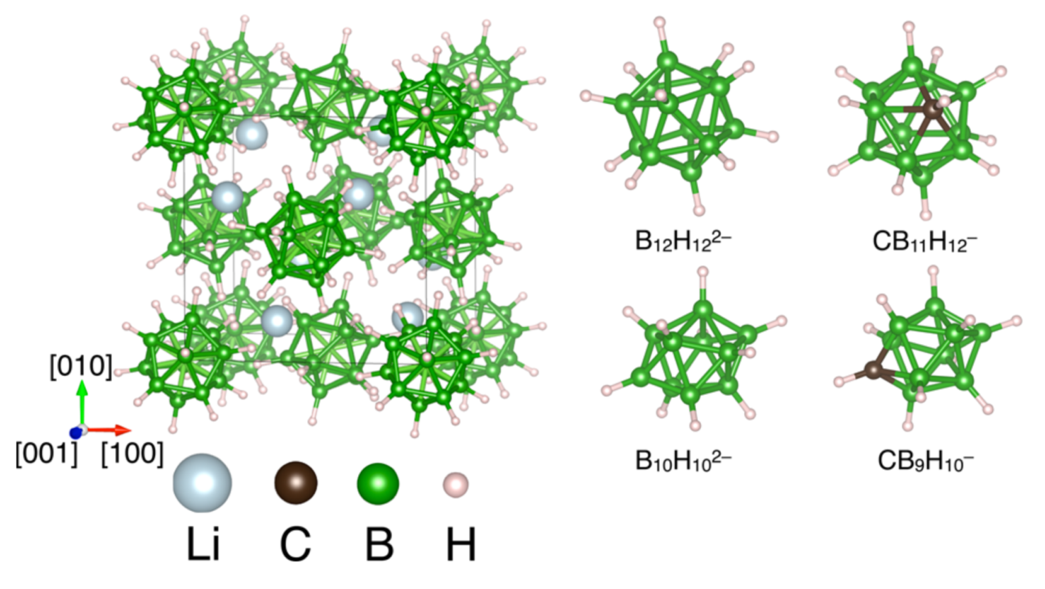
\includegraphics[width=0.7\textwidth]{\figurepath/batteries/polyborane_structure.png}
\caption{Crystalline \textit{fcc} structure of \ce{Li2B12H12} at room temperature.}
\label{batteries:fig-polyborane_structure}
\end{figure}

The high ionic conductivity of polyborane salts is believed to be connected to rapid reorientations of the anions~\cite{Skripov2015, Varley2016}, as well as the frustration between crystal symmetry and the local anion geometry as a result of long-range coulombic and short-range covalent-like interactions~\cite{Kweon2017}. Moreover, the lattice stacking of the large anions introduces spacious interstitial channels which facilitate cation conduction~\cite{Tang2015}, and because there are many more cation sites than cations, the structure can be interpreted as intrinsically high-vacancy, reducing the chance of migration channels being blocked. The interplay between the anion dynamics and cation mobility is complex, and I do not aim to provide a detailed explanation here. Instead, I will simply focus on my contribution to this line of research and its relation to other computational and experimental results. For more details, I refer the reader to the excellent analysis presented in the work of my collaborators~\cite{Varley2016, Kweon2017, Dimitrievska2018}.

\resultsubsection{Energy landscape of \ce{[CB11H12]^{-}} \label{batteries:sec-landscape}}{https://github.com/mbercx/phd-thesis/tree/master/jupyter/batteries\#energy-landscape-of-cb11h12-}{landscape}

In order to understand the local interaction between the anion and cation, I have calculated the energy landscape of the cation along a chain of ``wedges", i.e. curved 2D landscapes that connect the inequivalent facets of the anion (see Fig.~\ref{batteries:fig-cb11h12}(a), as well as Fig.~\ref{automation:fig-landscape}). This involves calculating the energy of the anion-cation system with a static calculation for many different cation positions around the anion. Moreover, in order to be able to reasonably compare the energy landscapes of \ce{Li^+} versus \ce{Na^+}, I have calculated a reference energy based on the average of a spherical landscape with a radius of 8~\si{\angstrom}. Besides giving a better idea of the binding energy of the cation-anion pair, this also provides a measure for how easily the cation is able to hop back to an interstitial site, as the \textit{fcc} lattices of \ce{LiCB11H12} and \ce{NaCB11H12} have similar lattice constants (9.936~\si{\angstrom} and 10.066~\si{\angstrom}, respectively~\cite{Tang2015}). All of the landscapes presented in this section are compared with respect to this reference energy. The workflow used to calculate the landscapes is described in Section~\ref{automation:sec-landscape}, the computational details can be found in \link{appendix:sec-landscape}{corresponding section} in Appendix~\ref{appendix:sec-results}.

{
\begin{figure}[ht]
\centering
\begin{tikzpicture}

\node at (0.065\textwidth,-0.5) {\textsf{\textbf{a}}};

\node [anchor=north west] at (0.06\textwidth, 0) {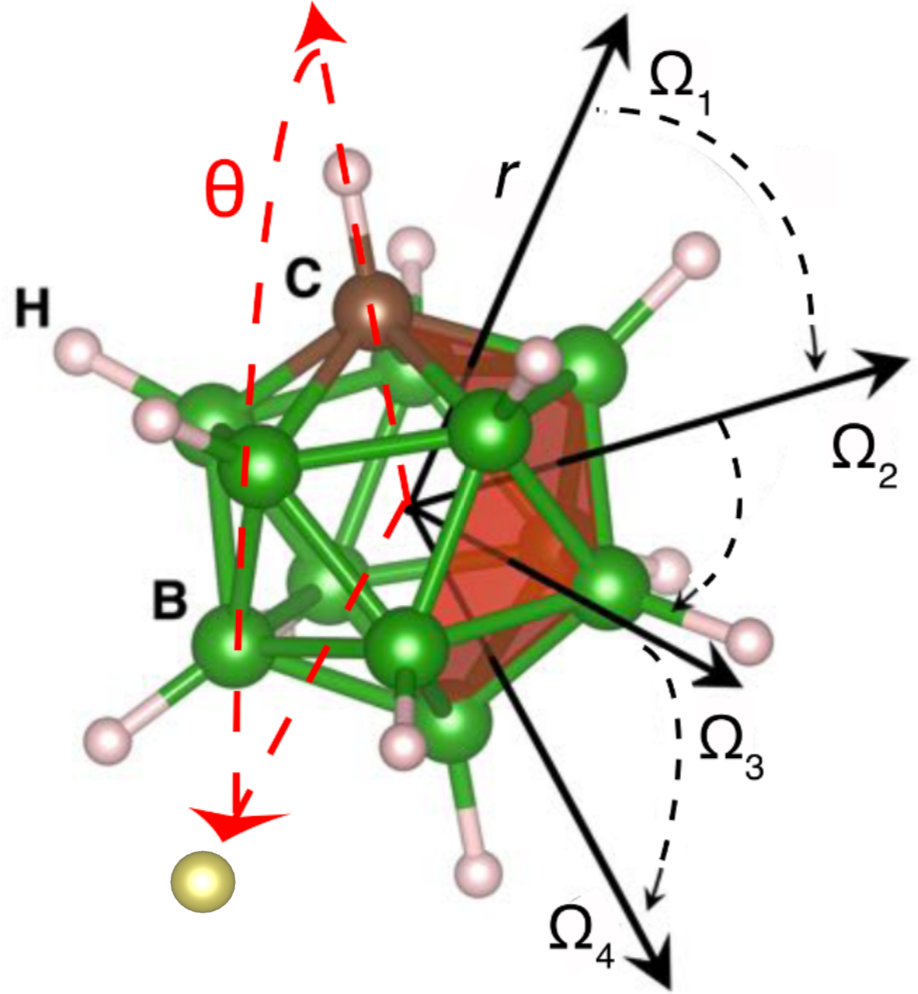
\includegraphics[width=0.31\textwidth]{\figurepath/batteries/anion_cb11h12.png}};

\node at (0.13\textwidth, -5.3) {\footnotesize \textsf{\textbf{Li/Na}}};

\node at (0.46\textwidth, -0.5) {\textsf{\textbf{b}}};

\node [anchor=north west] at (0.0\textwidth, -5.75) {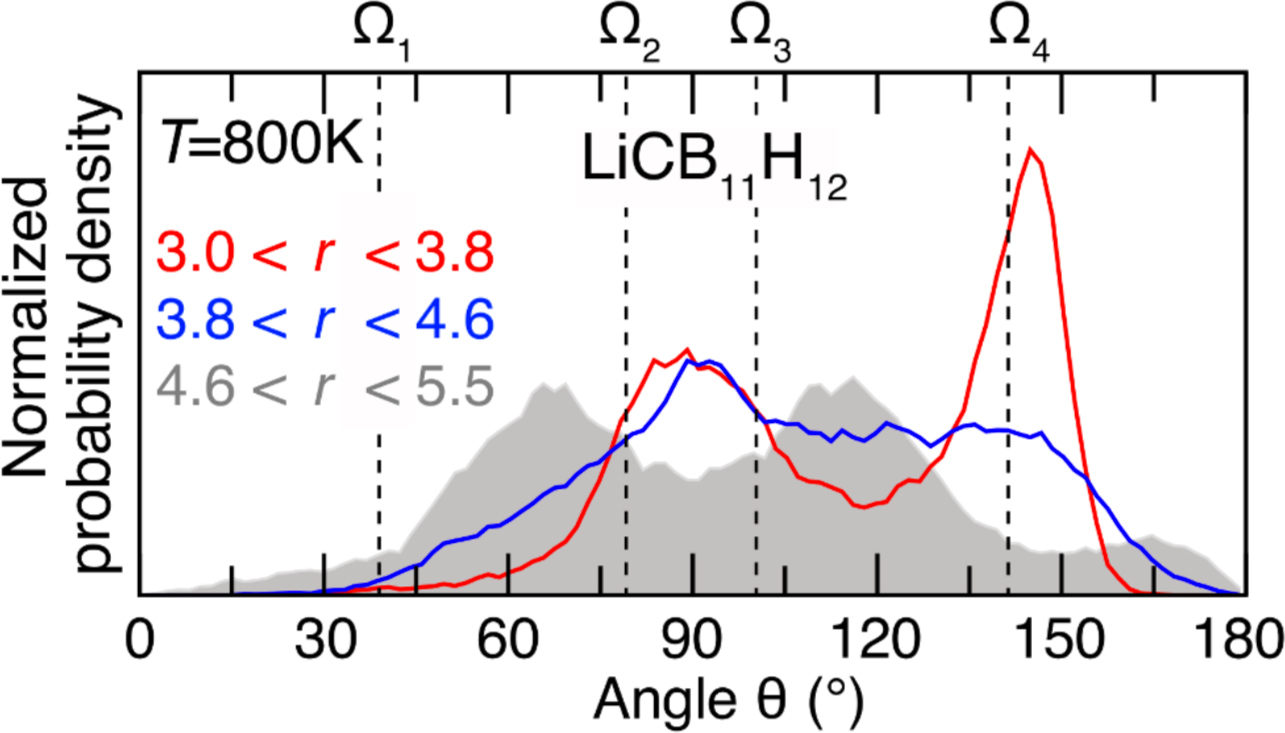
\includegraphics[width=0.44\textwidth]{\figurepath/batteries/aimd_cb11h12_Li.png}};

\node at (0.065\textwidth, -5.9) {\textsf{\textbf{c}}};

\node (landscapes) [anchor=north east] at (1.0\textwidth, -0.05) {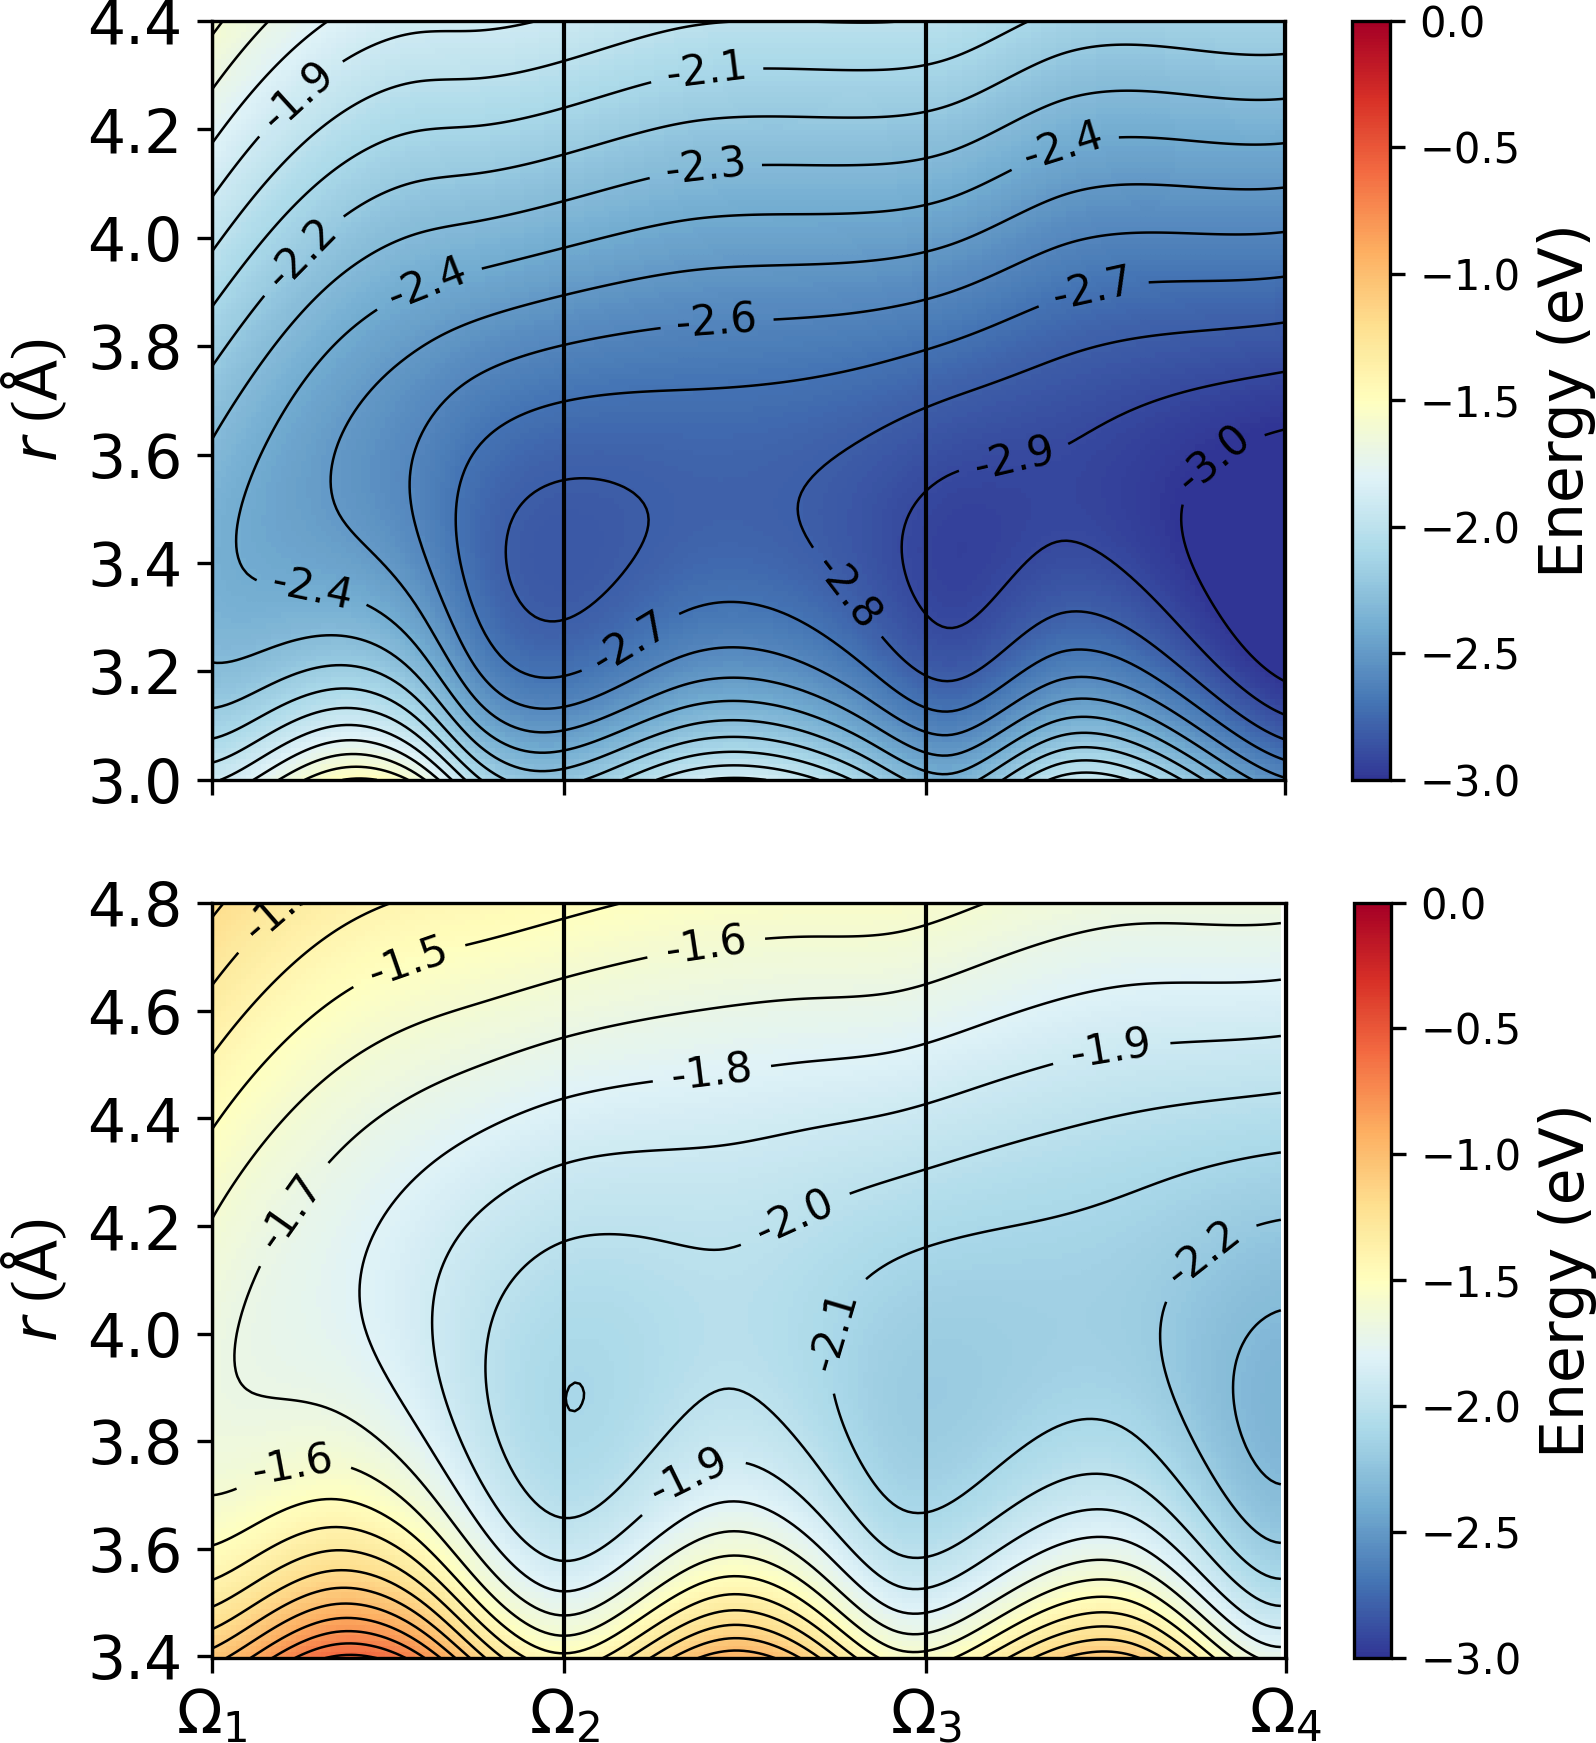
\includegraphics[width=0.54\textwidth]{\figurepath/batteries/ls_cb11h12.png}};

\node [fill=white, rounded corners, anchor=north west, font=\small\bfseries, text width=width("Na"), align=center] at (0.53\textwidth, -0.38) {\ce{Li}};

\node [fill=white, rounded corners, anchor=north west, font=\small\bfseries, text width=width("Na")] at (0.53\textwidth, -5.15) {\ce{Na}};


\end{tikzpicture}


\caption{(a) \ce{[CB11H12]^{-}} anion, with the symmetrically inequivalent facets colored red. Each of the facets corresponds to a binding site with direction $\Omega_i$ with respect to the center of the anion. (b) Angular distributions of the \ce{Li^+} (top) and \ce{Na^+} (bottom) cations derived from AIMD simulations (Taken from~\cite{Dimitrievska2018}), where the angle $\theta$ is defined versus the C$_5$ axis connecting the C atom with the opposite B atom. (c) Calculated energy landscapes for \ce{Li^+} (top) and \ce{Na^+} (bottom) along wedges connecting the binding sites $\Omega_i$, relative to the spherical average at $8~\si{\angstrom}$.}
\end{figure}
\label{batteries:fig-cb11h12}
}

The resulting energy landscapes are compared with the ab initio molecular dynamics (AIMD) results from Dimitrievska et al.~\cite{Dimitrievska2018} in Fig.~\ref{batteries:fig-cb11h12}. The landscapes of \ce{Li^+} and \ce{Na^+} are qualitatively similar, and show a preference for the cations to bind at all-boron facets, where the depth of the energy wells is progressively larger for sites further removed from the \ce{C} atom. This result is in good agreement with the angle distributions obtained from the AIMD, where we can see that the probability density is larger for angles corresponding to the all-boron docking sites ($\Omega_2$, $\Omega_3$ and $\Omega_4$), especially at smaller distances. At these distances, the likelihood of finding the cation near the $\Omega_4$ site is largest, which matches nicely with the increasing depth of the energy wells for sites further removed from \ce{C}. 

Moreover, the difference in the energy landscape between the \ce{C} facet ($\Omega_1$) and the lowest energy binding site ($\Omega_4$) is significant ($>0.6~\si{\electronvolt}$). As the anions undergo rapid reorientation in the superionic phase of both \ce{LiCB11H12} and \ce{NaCB11H12}~\cite{Dimitrievska2018}, this leads to a strongly fluctuating cation energy landscape close to the anions, which can push the cation back into interstitial sites. Hence, the substitution of \ce{B} by \ce{C} introduces a dipole in the anion, which in combination with its high rotational mobility can improve the ionic conductivitiy. This ``paddle wheel" effect was already described by Lunder et al. in the context of lithium sulphate materials~\cite{Lunden1995}, and is further supported by the by the AIMD and quasielastic neutron scattering results of my collaborators~\cite{Dimitrievska2018}. 

Comparing the results for \ce{Li^+} and \ce{Na+}, it is clear that the cation is bound less strongly for \ce{Na^+}, as the wells corresponding to the binding sites are much higher in energy compared to the reference at 8~\si{\angstrom}. Moreover, the wells are also broader and located at a larger distance from the anion, which further indicates that cation can more easily be detached from the anion. This, in combination with the fact that the energy difference upon reorientation of the anion is similar to that for \ce{Li^+}, can explain the lower transition temperature to the superionic phase for \ce{NaCB11H12} (380~\si{\kelvin}) compared to \ce{LiCB11H12} (400~\si{\kelvin}).

\pagebreak[4]
\section{Conclusions and Outlook} 

In this chapter, I have made a comparison of the stability of the oxygen 
framework of two layered oxide materials which are being investigated for use 
as a cathode in \ce{Li}-ion batteries. An extensive study of the optimal 
lithium configuration at different states of charge shows that when the 
\ce{Li2MnO3} cathode is charged by 75\%, the stacking changes from O3 to O1.
Based on the charged structure, a comparison of the stability of the oxygen 
framework indicates that the formation of O-O dimers is both thermodynamically 
and kinetically viable for O1-\ce{Li_{0.5}MnO3}. For O1-\ce{Li_{0.5}IrO3}, the 
oxygen lattice is much more stable, either returning to its original 
state when perturbed, or resulting in a structure with an O-O dimer that is 
much higher in energy. This can in part be explained by the mixed redox 
process for \ce{Li2IrO3}, which is also confirmed by the calculated magnetic 
moments and calculated change in projected density of states.

The lack of O-O dimer formation in O1-\ce{Li_{0.5}IrO3} suggests that introducing 
transition metals in the Li-rich structure which allow for higher states of 
oxidation is a reasonable path for reducing the likelihood of the formation of 
O-O dimers, and the corresponding structural changes of the cathode that are 
tied to the detrimental voltage fade and oxygen evolution. However, other 
research has also shown that \ce{Sn} substitution can improve the structural 
stability. We have studied the solubility of \ce{Sn} in the 
\ce{Li_{1.2}Mn_{0.8}O2} structure, and find that only a limited substitution 
is thermodynamically feasible. Based on these results, we decided to study 
the influence of a single substitution of \ce{Mn} by \ce{Sn}, \ce{V} 
or \ce{Mo} on the oxygen oxidation and stability of its framework. Our results 
indicate that substituting \ce{Mn} by \ce{Sn} does little to change the 
properties of the oxygen framework, most likely due to their similar 
chemical inactivity during the charging process. For \ce{V} and \ce{Mo}, the 
substitution does reduce the oxidation of the neighbouring oxygen atoms, 
but does not result in an improved stability. Instead, the kinetic barrier 
for dimerization is decreased further, indicating that the substitution 
destabilizes the structure instead. 

Although our results indicate that the formation of oxygen dimers in 
O1-\ce{Li_{0.5}MnO3} is likely to occur, we have yet to study its connection 
with the migration of Mn into the lithium layer. Other further investigations 
that could be interesting are the formation of oxygen dimers at the cathode 
surface, and subsequent evolution of \ce{O2} from the cathode into the 
electrolyte. So far, no substitution seems to be succesful at stabilizing 
the structure. However, other approaches have been suggested for 
increasing the cycling properties of Li-rich materials, such as \ce{Ni} 
substitution in the \ce{Li} layer~\cite{Yang2017}, or the substitution of 
oxygen by fluor~\cite{Richards2017, Kapylou2017}. Both make sense in the context of 
our results. The most likely dimer according to our analysis is formed 
across the \ce{Li} layer, which would be inhibited by the presence of \ce{Ni}. 
Fluor, on the other hand, does not oxidize \ce{Mn} as much, leaving more 
room for the transition metal to oxidize as \ce{Li} is removed from the 
cathode. Further research is necessary to see if these ideas can properly 
stabilize the Li-rich cathode, opening it up to further development and 
integration in commercial applications.

Finally, we have calculated the energy landscapes of \ce{Li^+} and \ce{Na^+} 
cations around the carbonated polyborane salt anion \ce{[CB11H12]^{-}}. From 
the landscapes, it is clear than substituting a single boron by carbon introduces 
a dipole in the anion molecule, which in combination with the rapid reorientations 
of the anions results in a paddle wheel mechanism that improves the ionic 
conductivity of the material. This suggests a novel strategy for improving 
the properties of these materials for solid-state battery applications.
 
\printbibliography

\end{refsection} 
